\documentclass[12pt]{report}
\usepackage[utf8]{inputenc}
\usepackage{graphicx}
\usepackage{amsmath}
\usepackage{SIunits}

\usepackage{caption}
\usepackage{subcaption}
\usepackage[margin=1in]{geometry}
\usepackage{url}
\graphicspath{ {Figures/} }
\bibliographystyle{unsrt}

\title{
	{Quantum Limited Gravitational Wave Detection}\\
	{\large University of Glasgow}\\
	{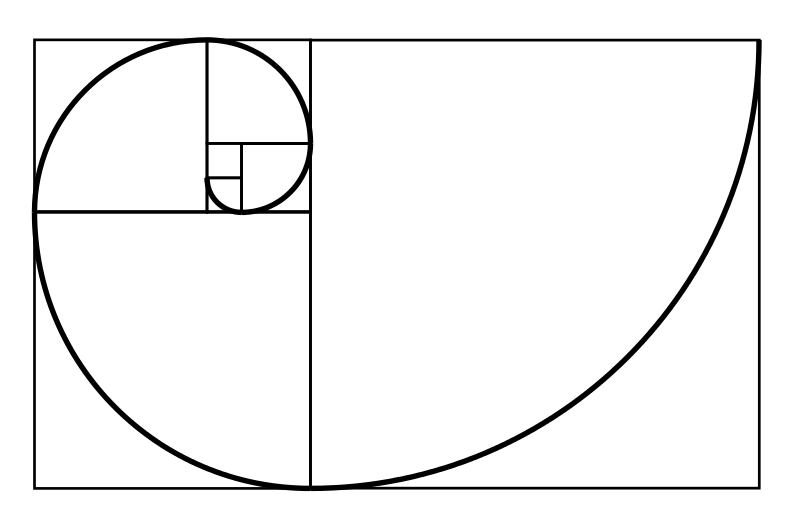
\includegraphics[width=0.5\textwidth]{place_holder.png}}
}
\author{Joseph Henry Briggs}
\date{Day Month Year}

\begin{document}
\maketitle

\chapter*{Abstract}
All you need are lasers and photodiodes. 

\chapter*{Dedication}

\chapter*{Declaration}
I declare that..

\chapter*{Acknowledgements}
I want to thank...

\tableofcontents

\chapter{Introduction}
This chapter should clearly motivate the need for gravitational wave measurements in the context of cosmology and astrophysics. It will (briefly) explain the types of sources that the detectors will be measuring (including a bit about LISA). It will talk about tests of general relativity, measurements of the age of the universe, multi-messenger measurements of the neutron star equation of state (its a combination of basically every field of physics), and so on... (I will read up more specific examples, but having large numbers of observations will tell us something about astrophysics). Although I'm not sure if I will mention dark matter in great depth, it probably deserves a mention since its one of the great mysteries of physics and gravitational wave detections may give insights into it. This will be an expanded version of the introduction to most papers written about gravitational wave detections, which hopefully will give you an idea of the tone of this chapter. It will be a relatively short chapter (about 5-10 pages?), but its vital in giving the rest of the work a reason to exist (some people do study graviational wave detectors as tools for probing the quantum nature of light, but most people will not see this as a good enough reason to spend billions of dollars developing them, heck not even everyone in the LVK collaboration thinks this is a good motivation for building the instruments!). Finally it will end with an explanation of each chapter in the thesis. This chapter will not cover the working principles of an interferometer
%\section{Introduction}
%\section{general relativity}
%\section{What is a gravitational wave}
%\section{How detections of gravitational waves have verified GR}
%\section{Sources of gravitational waves}
%formula for neutron star distance
%\section{how gravitational wave detections have been important to cosmology}
%\section{how gravitational wave detections have been important to astronomy}
%\section{thesis structure}

\chapter{Gravitational Wave Interferometers}
%This chapters purpose is to link general relativity to a basic michelson interferometer. I will keep the general relativity to a minimum, since this isn't a textbook on GR, however there is a small amount required to know why gravitational wave detectors are so big, why they are L shaped, etc. It will then expand on the basic michelson by adding the cavities. This is a good point to link sources to the detector, since the signal recycling adds shaping, its good to know why we aimed for 100Hz (I actually don't know why this was done, for some reason LIGO is optimised for detecting heavy black holes I think). Talk about noise sources, noise and senstivity curves, transfer functions between differential arm motion to light modulation at the AS port, mention the standard quantum limit. A detailed explanation of shot noise and radiation pressure noise should be in here, since these basically give you the requirements for the laser chapter and the photodiode chapter. Once the noise sources are covered, the BNS range can be shown. It makes sense to introduce the current detectors in more detail, and then talk about the 3rd generation of detectors. More novel topologies can be mentioned after. 
\section{Introduction}
The aim of this chapter is to outline some things about our universe we would like to know, how a gravitation wave allows this to be known, how an interferometer can be used to measure gravitational waves, the fundemental noise sources these detectors face. These noise sources can be reduced by making changes to the readout of the LIGO detector and by building new interferometers that use new technology. In this thesis, power of the laser and BHD is explored. Third generation detectors may operate at 2um, and so 2um detectors were characterised.
\section{Measuring Gravitational Waves}
\paragraph{general relativity (L shaped IFO)}
\paragraph{sources of GW}
\paragraph{observation runs and discoveries (detector hierarchy)}
\paragraph{The need for increasing detections...}
\section{Sources of noise when detecting gravitational waves}
\paragraph{shot noise and laser power}
\paragraph{quantum efficiency}
\paragraph{power recycling}
\paragraph{signal recycling to shape quantum noise}
\paragraph{squeezed light}
\paragraph{frequency dependent squeezing}
\paragraph{radiation pressure noise?}
\paragraph{other topologies of detectors}
\paragraph{other noise sources}
\section{The future of gravitational wave detectors}
\paragraph{cyro}
\paragraph{silicon}
\paragraph{2um or 1550}
\section{conclusion}
\begin{figure}
	\centering
	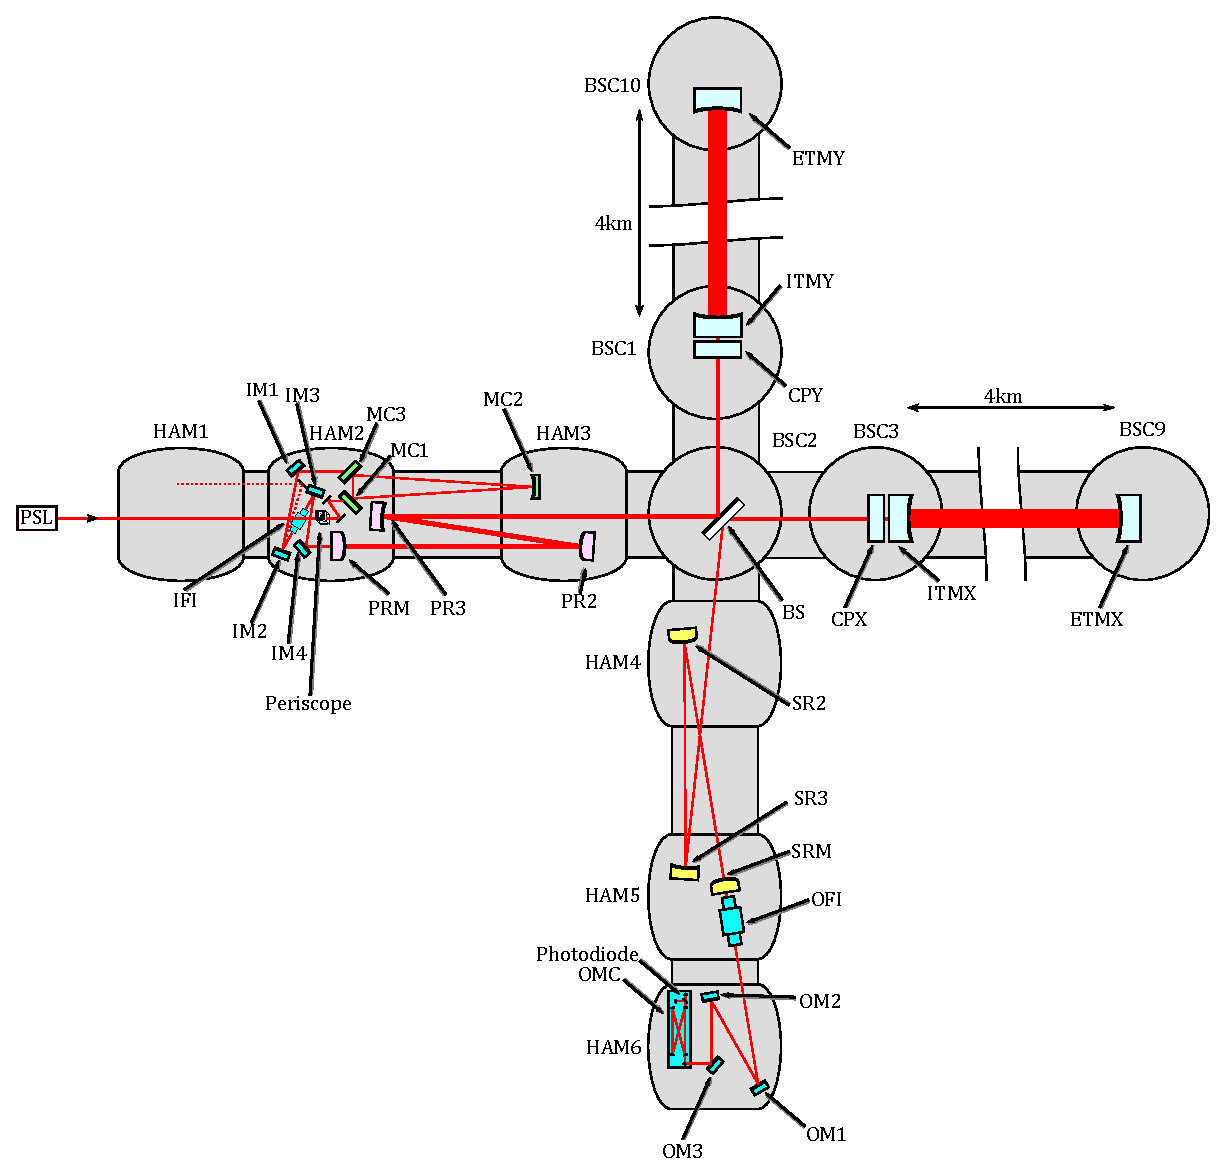
\includegraphics[width=1\linewidth]{Figures/LIGO_layout}
	\caption{}
	\label{fig:ligolayout}
\end{figure}

\chapter{High Power Laser Prototype for LIGO}
\section{Introduction}
\begin{itemize}
	\item why ligo needs high power
	\item brief history of LIGO laser 
	\item mention noise problems leading to wanting new amplifier
\end{itemize}
\section{Requirements}
\begin{itemize}
	\item power requirements
	\item long term stability requirement
	\item noise requirements (pointing+frequency+amplitude, only measured frequency and amplitude)
\end{itemize}
\section{OEM solid-state Amplifier}
\begin{itemize}
	\item why are they better than an HPO in principle
	\item how they work
	\item neovan 4S-HP
\end{itemize}
\section{Set-up and Layout}
\begin{itemize}
	\item diagram of layout
	\item description of layout
	\item use 2 amplifiers and a PMC to get high power gaussian beam
	\item flow rates and beam quality of amplifiers
\end{itemize}
\begin{figure}
	\centering
	\includegraphics[width=\linewidth]{figures/E1900168-v3_O4laser_TNT_TableLayout_AOM}
	\caption{e1900168. Layout placeholder}
	\label{fig:e1900168-v3o4lasertnttablelayoutaom}
\end{figure}

\section{Frequency Noise}
Need to put together the measurements for frequency noise.
\begin{figure}
	\centering
	
\includegraphics[width=0.7\linewidth]{figures/PMC_open_loop_transfer_function}
	\caption{Open loop gain of frequency stabilisation loop}
	\label{fig:pmcopenlooptransferfunction}
\end{figure}
\section{Long Term Power Results}
In touch with Matt about his, I would like 1 month or something like that (as long as possible)
\begin{figure}
	\centering
	
\includegraphics[width=0.7\linewidth]{figures/mode_scan_comparisons}
	\caption{Flow rates affecting the thermal lensing, resulting in increased ellipticity}
	\label{fig:modescancomparisons}
\end{figure}

\section{Conclusion}
summary of how much power for how long, and how it could be improved slightly with mode matching
\chapter{Amplitude Stabilisation for High Power Laser at LIGO}
\section{Introduction + Requirements}
\begin{itemize}
	\item shot noise requirement
	\item radiation pressure noise setting noise requirement
	\item inner+outer loop design
	\item could include calculation for mismatches in the IFO? Point absorbers etc.
\end{itemize}
\section{Free Running Noise and Noise Hunting}
\begin{itemize}
	\item free running noise of the laser
	\item what dominates the laser noise? NPRO
	\item noise sources such as mounts 
	\item noise from PMC offset not being tuned
	\item 4Hz noise from Beckhoff
\end{itemize}
\section{AOM Stabilisation}
\begin{itemize}
	\item description of AOM
	\item AOM TF
	\item AOM loop TF
	\item plot of AOM stabilisation working
\end{itemize}
\begin{figure}
	\centering
	
\includegraphics[width=0.7\linewidth]{figures/AOM_stabilisation_noise}
	\caption{Free running and stabilised noise of laser}
	\label{fig:aomstabilisationnoise}
\end{figure}
\begin{figure}
	\centering
	
\includegraphics[width=0.7\linewidth]{figures/AOM_stabilisation_TF}
	\caption{Transfer functions for parts of the AOM servo}
	\label{fig:aomstabilisationtf}
\end{figure}
\section{Current Shunt Stabilisation}
\begin{itemize}
	\item description of CS
	\item CS TF
	\item CS loop TF
	\item plot of CS stabilisation working
\end{itemize}
\begin{figure}
	\centering
	
\includegraphics[width=0.7\linewidth]{figures/current_shunt_tfs}
	\caption{current shunt input to light power transfer function for different diode currents}
	\label{fig:currentshunttfs}
\end{figure}
\begin{figure}
	\centering
	
\includegraphics[width=0.7\linewidth]{figures/dc_power_all_pd}
	\caption{DC behaviour of current shunt}
	\label{fig:dcpowerallpd}
\end{figure}
\section{Comparison of Two stabilisation Schemes}
\begin{itemize}
	\item why I think the AOM is a better choice even though they both work
\end{itemize}
\section{Conclusion}
\chapter{Balanced Homodyne for LIGO A+}
\textcolor{red}{There doesn't need to be a discussion about what BHD is, but it is worth briefly mentioning what it is and the other readout methods again}
Context for BHD upgrade being part of A+. 
\section{BHD versus DC readout for A+}
\begin{itemize}
	\item \href{https://dcc.ligo.org/G2000962}{G2000962}, DDR CDR presentation A.	
	\item \href{https://dcc.ligo.org/LIGO-G2001026}{G2001026}, DDR CDR presentation B.
	\item Ken's notes on BHD benefits compared to DC readout, email on 25/06/2020 11:26
	\item \href{https://dcc.ligo.org/LIGO-L2000200}{LIGO-L2000200} Q and A. Useful technical points and things people will find confusing/may ask about.
\end{itemize}
\paragraph{}
Main benefit of BHD is reduction of SRC length noise coupling to AS port. This noise coupling is described in \cite{Izumi2016}, see equation 13. This paper has some coupled cavity maths in it. If this needs explained, look up \href{https://dcc.ligo.org/LIGO-P000013}{Transfer Functions for Fields in a 3-Mirror Nested Cavity}, \cite{Rakhmanov2000}. There is an opto-mechanical coupling between the length of the SRC and arm cavity (due to radiation pressure). Reducing the DC offset reduces the radiation pressure, which reduces this coupling.
\paragraph{estimate reduction of SRC length noise coupling}
Equation for SRC length noise to AS signal is (I couldn't get this to plot, need to debug this)
\begin{equation}
	\frac{S_{\rm{as}}}{S_{\rm{dc}}} = 4g_p^2g_s^2r'^2_a \epsilon\left(\frac{\partial L_-}{\partial l_s}\right)\frac{k\Delta l_s}{1+s_{\rm{rse}}}
\end{equation}
the TEM00 is decreased to fringe offset (rms + DC) + 1mW of common mode carrier, currently there is 20mA of photo-current. (shelia dwyer answer in email FW: BHD review committee request \& document PREVIEW).
\section{Derivation of path length stability}
\begin{itemize}
	\item \href{https://dcc.ligo.org/LIGO-G1702485}{Hang Yu BHD requirements}
\end{itemize}
\paragraph{}
Analytic expression
\cite{Izumi2016} and finesse simulation.
\section{WS visulations as a tool for understanding mode matching problems}
\section{Mode matching with astigmatism}
\section{Algorithm for calculating optimal 3 lens mode matching solution}
\section{HAM6 layout}
\section{Thermal lensing}
\section{Arm cavity power linked to AWC}
\section{Conclusion about BHD for A+}

\chapter{in Air BHD experiments}
%A Michelson interferometer converts a change in optical path length into a change in intensity of light. Shot noise is one of the fundamental limits on how precisely the path length can be known. As shot noise manifests as intensity fluctuations of the light, it is indistinguishable from intensity fluctuations that arise due to the differential phase modulation of interfering beams.
%\par
In this Chapter, it is demonstrated that the shot noise measured with the transimpedance amplifier developed for some of the experiments in Chapter~\ref{chapter:2um_photoiode_chapter} can be used to measure shot noise within an interferometer, thus linking the shot noise of a current to the phase of light. To do this, a Mach-Zehnder interferometer was used. This also makes the experiment topologically similar to a Michelson interferometer with a balanced homodyne detection scheme. A shot noise limited measurement was made in-air, and this is reported in Section~\ref{sec:MZ_chapter_in_air}. Section~\ref{sec:MZ_chapter_in_vac} is a description of an attempt to perform this measurement in-vacuum so that shot noise could be measured at lower frequencies, however due to scattered light, this was unsuccessful.
\section{Shot Noise in a Mach-Zehnder Interferometer}
\label{sec:MZ_chapter_in_air}
A sketch of a Mach-Zehnder interferometer is shown in Figure~\ref{fig:mzchaptermzsketch}. At the second beam splitter, two beams are combined to produce an interference pattern that depends on the relative phase between the two beams. This is analogous to an interferometer that uses balanced homodyne detection. In an interferometer with a balanced homodyne detection scheme, the two beams are called the signal and local oscillator.
\par
The difference between a Mach-Zehnder interferometer and a Michelson interferometer with a balanced homodyne detection scheme is what the phase of the signal beam means. In a Mach-Zehnder interferometer, the phase corresponds to the motion of a mirror whereas in a Michelson interferometer with a balanced homodyne detection scheme, the phase corresponds to a differential motion of the ETMs.
\begin{figure}
	\centering
	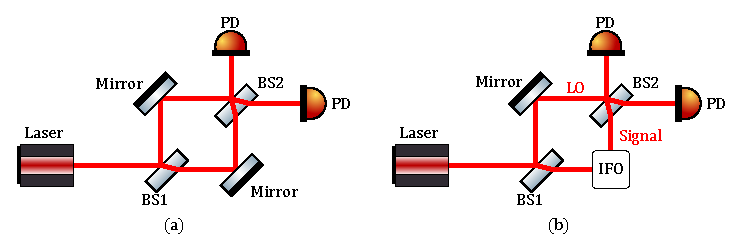
\includegraphics[width=1\linewidth]{Figures/MZ_chapter_mz_sketch}
	\caption{(a) Sketch of a Mach-Zehnder interferometer. The interference at BS2 depends on the difference in the phase of the two beams after BS1. (b) Sketch of an interferometer (IFO) with a balanced homodyne detection scheme. A Michelson interferometer adds a phase modulation to the signal beam, and this results in an intensity modulation in the combined beams after BS2. In essence, (b) is similar to (a).}
	\label{fig:mzchaptermzsketch}
\end{figure}
\par
The signal measured by each photodiode can be described by Equation (\ref{eq:bhdforligo_interference_at_a_beam_splitter}). The shot noise of this measurement depends on the total amount of light in the signal and LO beam, and because the power of the LO beam, $P_{\rm{LO}}$, was much greater than the power of the signal beam, $P_{\rm{sig}}$, the amplitude spectral density associated with the shot noise, $n_z$, of the detected light can be expressed in units of $\si{\metre_{\rm{rms}}/\sqrt{\hertz}}$ by
\begin{equation}
n_z = \sqrt{\frac{2hc\lambda}{16\pi^2P_{\rm{sig}}}}
\label{eq:MZ_chapter_shot_noise_level}.
\end{equation}
The noise, $n_z$, can be interpreted as the detected amount of relative motion between the two mirrors in the Mach-Zehnder interferometer. 
\subsection{Apparatus for the In-Air Mach-Zehnder.}
The in-air Mach-Zehnder is shown in Figure \ref{fig:mzchapterinairmz} and Figure \ref{fig:mzchapterinairsketch}. It was constructed from highly stable, rigid mounts to keep the noise due to the vibration of the mounts low. The Mach-Zehnder was mounted on a thick aluminium base-plate which was isolated from the optical table by rubber dampeners. The Mach-Zehnder was acoustically shielded with a plastic box of a $\sim1\si{\milli\metre}$ thickness. A half-wave plate and polarised beam splitter were used to control the power entering the Mach-Zehnder and the polarisation of the light entering the Mach-Zehnder.
\begin{figure}
	\centering
	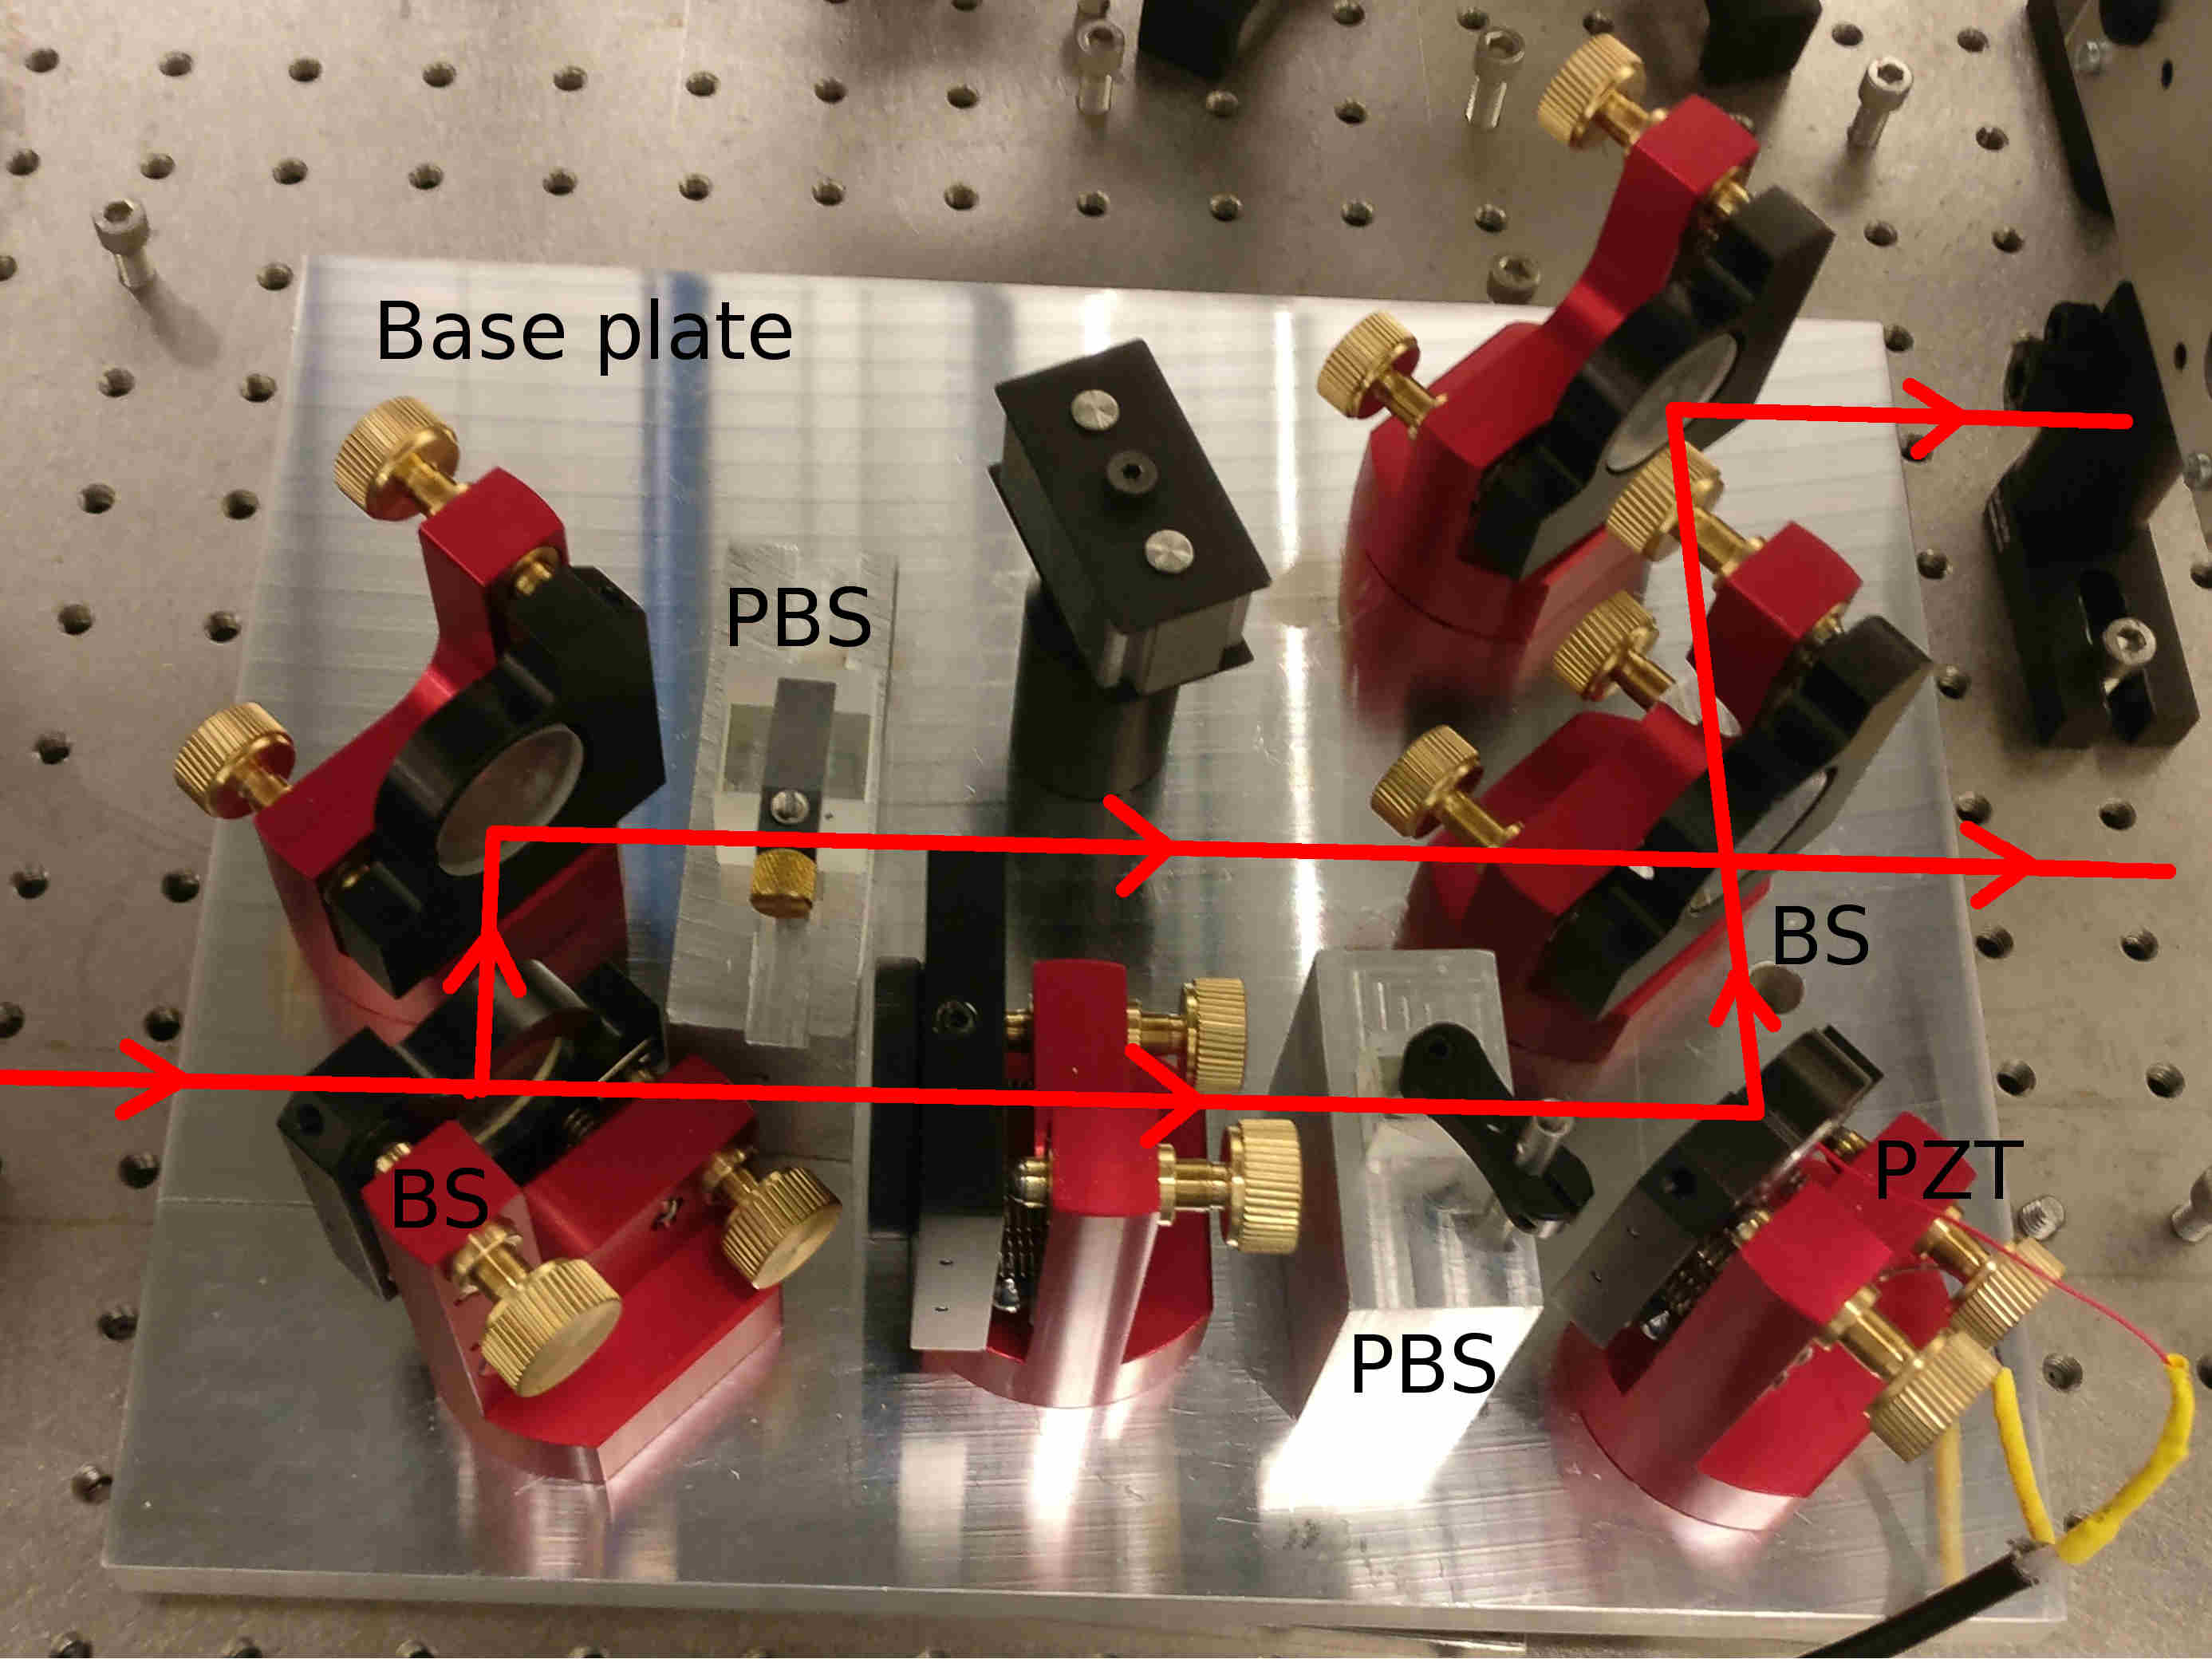
\includegraphics[width=0.7\linewidth]{Figures/MZ_chapter_in_air_MZ}
	\caption{Photograph of the Mach-Zehnder base plate. The polarising beam splitters were part of an earlier design; they were removed when the measurements with this apparatus were made. }
	\label{fig:mzchapterinairmz}
\end{figure}
\begin{figure}
	\centering
	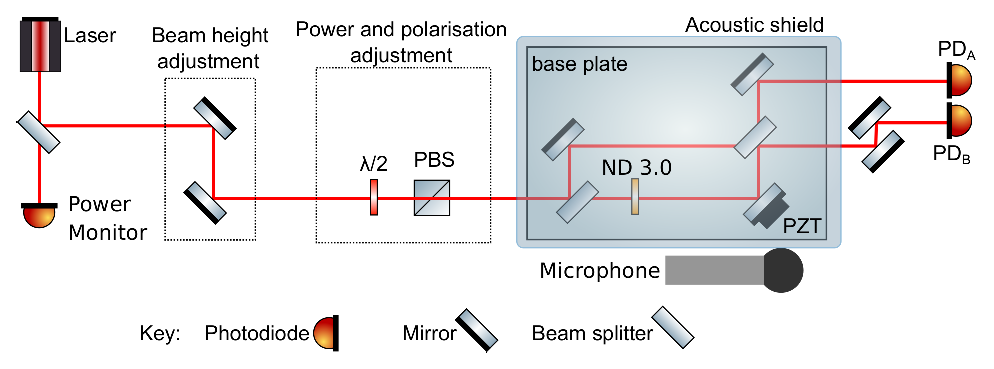
\includegraphics[width=1\linewidth]{Figures/MZ_chapter_in_air_sketch}
	\caption{Sketch of the optical layout. The laser was generated by an NPRO. The power of the laser was monitored using a photodiode immediately after the laser. The beam's power and polarisation were controlled with a half wave plate and polarising beam splitter (PBS). The Mach-Zehnder was mounted on a base plate, and it was acoustically shielded by a plastic box and rubber feet. The splitting ratio of the BS2 was measured to be 50:50. An ND filter was used to decrease the power in one of the paths within the Mach-Zehnder. }
	\label{fig:mzchapterinairsketch}
\end{figure}
\par
The reflectivity, $R$ and transmissivity, $T$, of the beam splitter on which the beams were recombined was measured to be $0.5\pm0.01$. To replicate a situation analogous to a balanced homodyne detection scheme, the power in one arm was attenuated. The beam size within the Mach-Zehnder was small, so the light power in one arm was attenuated with an ND filter as surface roughness of the ND filter did not matter. The optical density of the ND filter was found by measuring the ingoing and outgoing beam's power with $\rm{PD_A}$ and $\rm{PD_B}$; this was done by blocking the upper path and measuring the signal with and without the ND filter. The ND filter decreased the power in the signal arm by a factor of 232.
\par
The signals from the photodiodes were measured using the same design of transimpedance amplifier as in the experiment in Section~\ref{sec:pd_chapter_reverse_bias_qe}. This design gives sufficient SNR to make shot noise limited measurements for currents $\sim20\,\si{\milli\ampere}$. The design of this amplifier is shown in~Appendix \ref{sec:circuits_appendix_variable_bias_ad797}. The response of this photodiode circuit is flat at all frequencies of interest and is 390\,V/W at DC. 
\par
The signals from the photodiodes were recorded with CDS (see Appendix~\ref{app:CDS}). Voltages that are measured with CDS are quantised by analogue-to-digital (ADC) converters. Each quanta is called a \emph{count}. The ADCs have 16 bits, and the peak-to-peak voltage that the ADC can record is 20\,V, so the relationship between the input voltage to CDS and a count is $20/(65536)$. CDS features an anti-aliasing filter which affects measurements above $9\,\si{\kilo\hertz}$. The response of the AA filter can be seen in Figure \ref{fig:mzchaptercdsnoise}.
\par
Cables are susceptible to common-mode noise that arises due to pick up. To avoid this problem, the signals were sent differentially to CDS. Send-receive circuits were constructed with the THAT range of IC. A by-product of using these send-receive circuits was the signals from the photodiodes were multiplied by a factor of two.
\par
To keep the measured signal above the digitisation noise inherent to the ADCs used in CDS,  whitening filters are required.  CDS noise is shown in Figure \ref{fig:mzchaptercdsnoise}. A whitening circuit boosts the AC components of a signal while keeping the DC level of the signal small enough as to not saturate CDS's ADCs. A dewhitening filter is a digital filter whose transfer function is the reciprocal of the whitening filter's transfer function.  For this photodiode circuit, the level of shot noise due to 20\,mW of light is $\sim3\times10^{-8}\,\rm{V_{rms}/\sqrt{Hz}}$ and so the whitening filter needs to boost the photodiode signal by 40\,dB. The transfer function of the electronics for sending, receiving and whitening the photodiode signal is shown in Figure \ref{fig:mzchapterinairsendrecievefilter}.
\begin{figure}
	\centering
	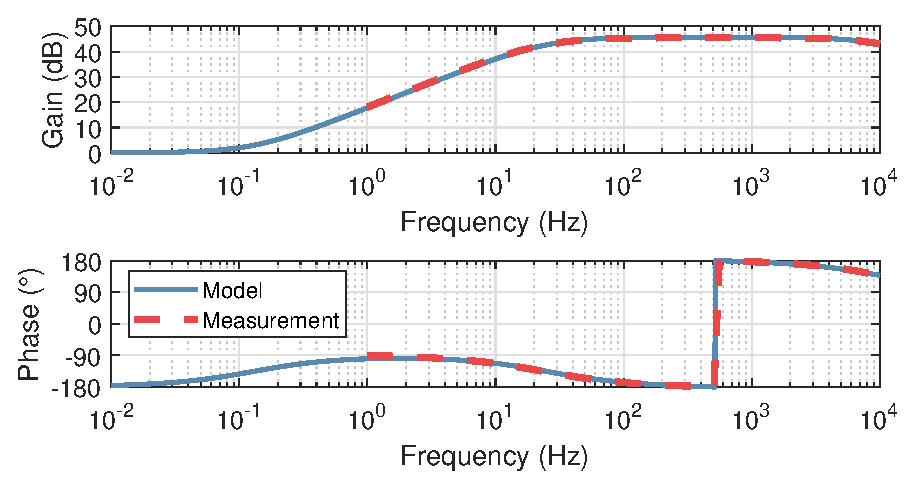
\includegraphics[width=1\linewidth]{Figures/MZ_chapter_in_air_send_recieve_filter}
	\caption{The transfer function of the electronics for sending, receiving and whitening the photodiode signal was modelled and measured. This gave the desired level of SNR to make shot noise limited measurements above $\sim200\,\rm{Hz}$.}
	\label{fig:mzchapterinairsendrecievefilter}
\end{figure}
\par
A servo was required to lock the Mach-Zehnder to $<1\%$ of a fringe. The circuit diagram for the servo is shown in Figure \ref{fig:mzinairservocircuit}. The phase between the two beams was actuated on with by moving one of the corner mirrors with a PZT. The error signal was obtained by subtracting the signals from the two photodiodes. The error signal was low pass filtered, and the corner frequency of the low pass filter was at 1\,Hz. The PZT needed to be driven with a high voltage ($\sim100\si{\volt}$), so a high voltage op amp (OPA454) was used in the final stage of the servo electronics. The PZT had a capacitance, so the output of the OPA454 was followed by a resistor to prevent the op amp oscillating. This corresponded to an additional corner frequency in the servo at $\sim8\,\si{\kilo\hertz}$. To prevent the servo oscillating due to this additional pole, the overall gain of the servo was controlled with a potentiometer. A way of injecting signals onto the PZT was included in the servo. 
\begin{figure}
	\centering
	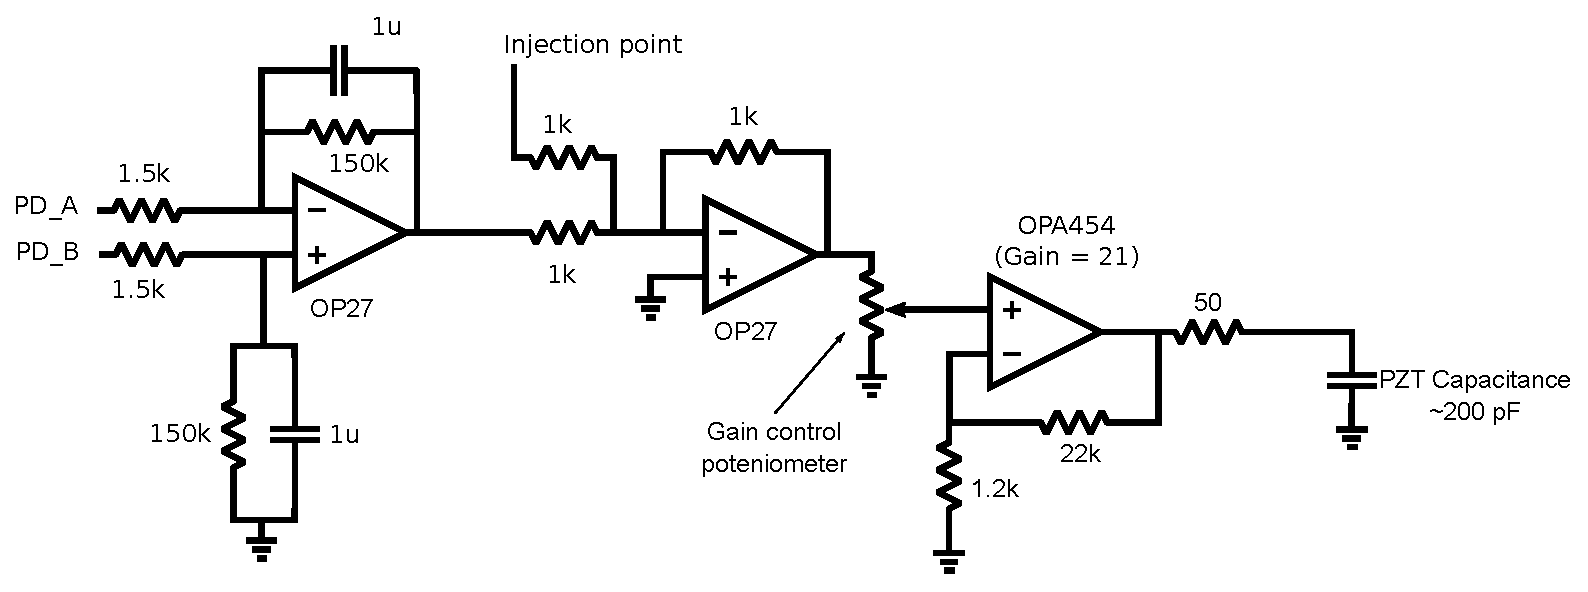
\includegraphics[width=1\linewidth]{Figures/MZ_in_air_servo_circuit}
	\caption{Circuit diagram for the electronics used to keep the in-air Mach-Zehnder locked to the middle of a fringe. The first stage subtracts the signals from the photodiodes and provides a 1\,Hz roll-off. The second stage allowed for a signal to be applied to the PZT. The final stage boosted the signal to around 100V. The final resistor was used to prevent the OPA454 oscillating.}
	\label{fig:mzinairservocircuit}
\end{figure}
\subsection{Calibration}
\label{sec:mz_chapter_in_air_cal}
The signal measured at the photodiodes can be calibrated in terms of the difference in path length between the two arms by applying a ramp signal to the PZT. Ramping the PZT causes the Mach-Zehnder to be driven over multiple fringes. The ramp signal and the photodiode signals were recorded on an oscilloscope. The difference in the photodiode signals was then plotted against the measured ramp signal. One period of this signal corresponds to one wavelength, so fitting a sinusoid to the data and finding its gradient around where the subtracted photodiode signal is 0\,V gives one the photodiode signal to path length conversion. This is shown in Figure~\ref{fig:mzchapterinaircalibration}. This measurement was affected by the quantisation noise of the oscilloscope.
\par
Alternatively, on can calibrate the differential path length signal by measuring the power in the two beams while they are not interfering (see Equation~(\ref{eq:bhdforligo_interference_at_a_beam_splitter})). The power of the LO beam was measured to be $20.3\pm0.1,\si{\milli\watt}$. Without the ND filter, the power of the signal beam was measured to be $18.3\pm0.1\,\si{\milli\watt}$, so with the ND filter it would be 78\,\si{\micro\watt}. This calibration is shown in Figure~\ref{fig:mzchapterinaircalibration}, and it agrees with the calibration obtained via ramping the PZT voltage to within 10\%.
\begin{figure}
	\centering
	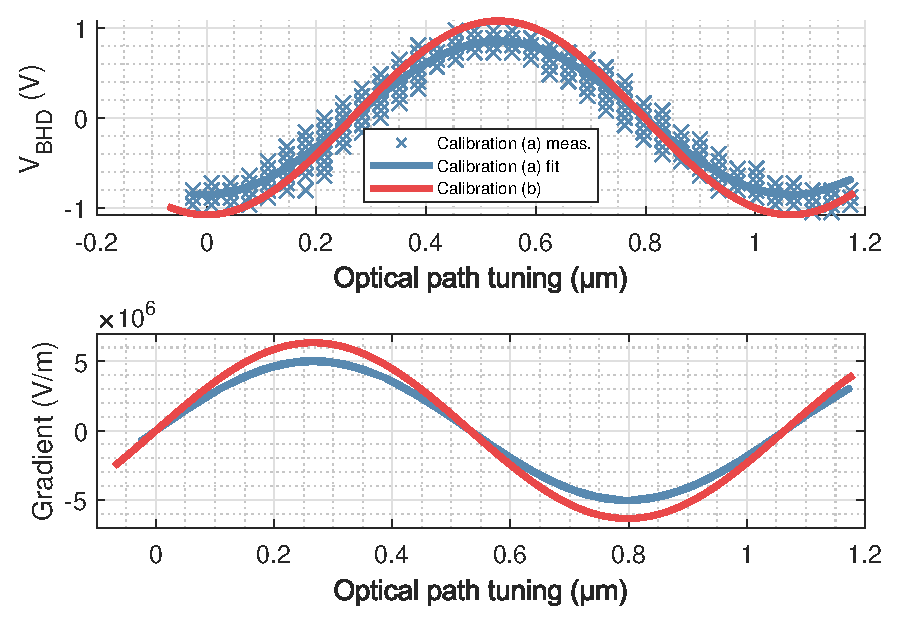
\includegraphics[width=1\linewidth]{Figures/MZ_chapter_in_air_calibration}
	\caption{There are two ways of calibrating the differential photodiode signal that will be generated by a change in optical path length between the two paths in the Mach-Zehnder. Method (a) is to measure a ramp signal that is applied to the PZT while simultaneously measuring the photodiode signals. The measurement of this is shown by the blue crosses, and the fit to this data is shown by the blue line. Method (b) is to measure the power in the local oscillator and signal beams when they are not interfering. From this, Equation~(\ref{eq:bhdforligo_interference_at_a_beam_splitter}) can be used to find the response of the Mach-Zehnder. This is shown by the red line. Thus, the blue and red data are independent of each other. The two calibrations agree to within 10\%. The gradient of $V_{BHD}$ is used to get the conversion factor for a change in beam power to a change in differential path length.}
	\label{fig:mzchapterinaircalibration}
\end{figure}
\subsection{Measurement of Shot Noise}
The Mach-Zehnder was locked, and the difference between the photodiode signals was measured. To demonstrate that the difference in the photodiode signals depended on the differential path length of the Mach-Zehnder, a modulation at 6033\,Hz was applied to the PZT. The amplitude spectral density of the difference in the photodiode signals is shown in Figure~\ref{fig:mzchapterfullnoisespectrum}. The signal was calibrated using the ramp technique described in Section~\ref{sec:mz_chapter_in_air_cal}. The dashed red line indicates the noise predicted by Equation~\ref{eq:MZ_chapter_shot_noise_level}, and at frequencies free of noise due to acoustic vibrations, this matches the measured noise to within 5\%. Thus, the measurement was limited by shot noise.
%\begin{table}
%	\centering
%	\begin{tabular}{|c|c|}
%		\hline
%		Parameter & Value \\
%		\hline
%		Nyquist Frequency & 32768\,Hz\\
%		Frequency Resolution & 10\,Hz \\
%		Effective Noise bandwidth & 15\,Hz\\
%		Number of Averages & 459 \\
%		\hline 
%	\end{tabular}
%\caption{A Hanning window was used to average the data and generate the amplitude spectral density. }
%\end{table}
\begin{figure}
	\centering
	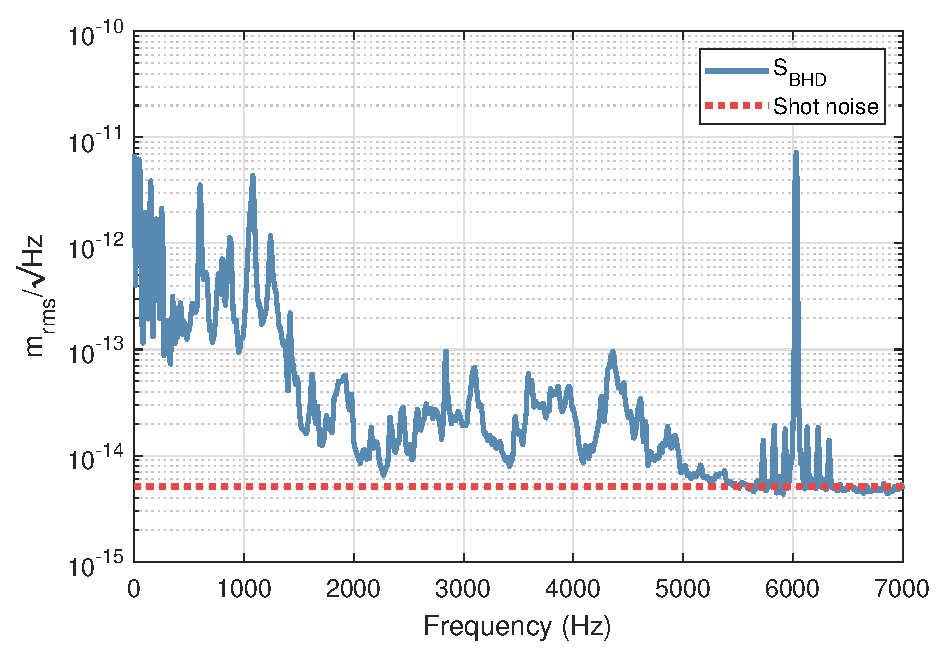
\includegraphics[width=1\linewidth]{Figures/MZ_chapter_full_noise_spectrum}
	\caption{The amplitude spectral density of the difference between the two photodiode's signals ($\rm{S_{BHD}}$) is shown in blue. The peak at 6033\,Hz was injected to demonstrate this measurement corresponds to differential arm length modulations. The expected shot noise is based on Equation~(\ref{eq:MZ_chapter_shot_noise_level}), and this is shown by the dashed red line. The noise measured at frequencies above 5500\,Hz is within 5\% of the expected shot noise. Below 5500\,Hz, acoustic noise limited the Mach-Zehnder's sensitivity.}
	\label{fig:mzchapterfullnoisespectrum}
\end{figure}
\section{Noise in an In-Vacuum Mach-Zehnder Interferometer and the Effect of Misalignment the Local Oscillator and Signal Beam}
\label{sec:MZ_chapter_in_vac}
To measure shot noise at frequencies around 100\,Hz, the frequency band of interest in a gravitational wave detector, the acoustic and seismic noise noise which shake the mirrors need to be reduced. This can be achieved by using suspended optics and performing the experiment in-vacuum. There was an opportunity to perform this experiment in-vacuum with left-over apparatus from a previous experiment. This proved challenging for as the interferometer was hard to lock due to large amounts of seismic motion coupling to the differential arm length. Ultimately, scattered light interfering with the differential arm signal meant that shot noise could not be measured at any frequency. However, this apparatus could be used to explore how misalignment will cause the signal to size to drop. 
\subsection{Apparatus for the In-Vacuum Mach-Zehnder}
A mach zehnder was constructed from suspended optics and placed in vacuum; this is shown in Figure \ref{}. The suspensions used were double pendulums of with masses of 75\si{\gram} separated by whiles of lengths 100\,mm (top to middle mass) and 150\,mm (middle to bottom mass), resulting in them having longitudinal resonances around $\sim 1$ \cite{Jans thesis}. The balanced homodyne readout platform (BHRP) was a suspended assembly that included the recombination beam splitter, steering mirrors for the recombined beams and photodiode. This photodiode circuit was the same as the one described in Section \ref{}. The vacuum system was pumped down to 1,mbar \ref{}. An NPRO was used to provide the laser light. 
\begin{figure}
	\centering
	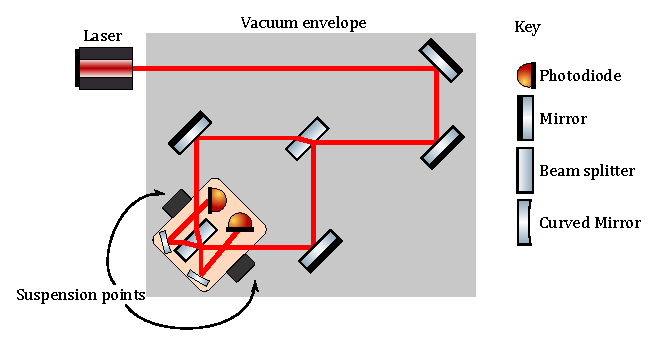
\includegraphics[width=1\linewidth]{Figures/MZ_chapter_in_vacuum_sketch}
	\caption{}
	\label{fig:mzchapterinvacuumsketch}
\end{figure}
\begin{figure}
	\centering
	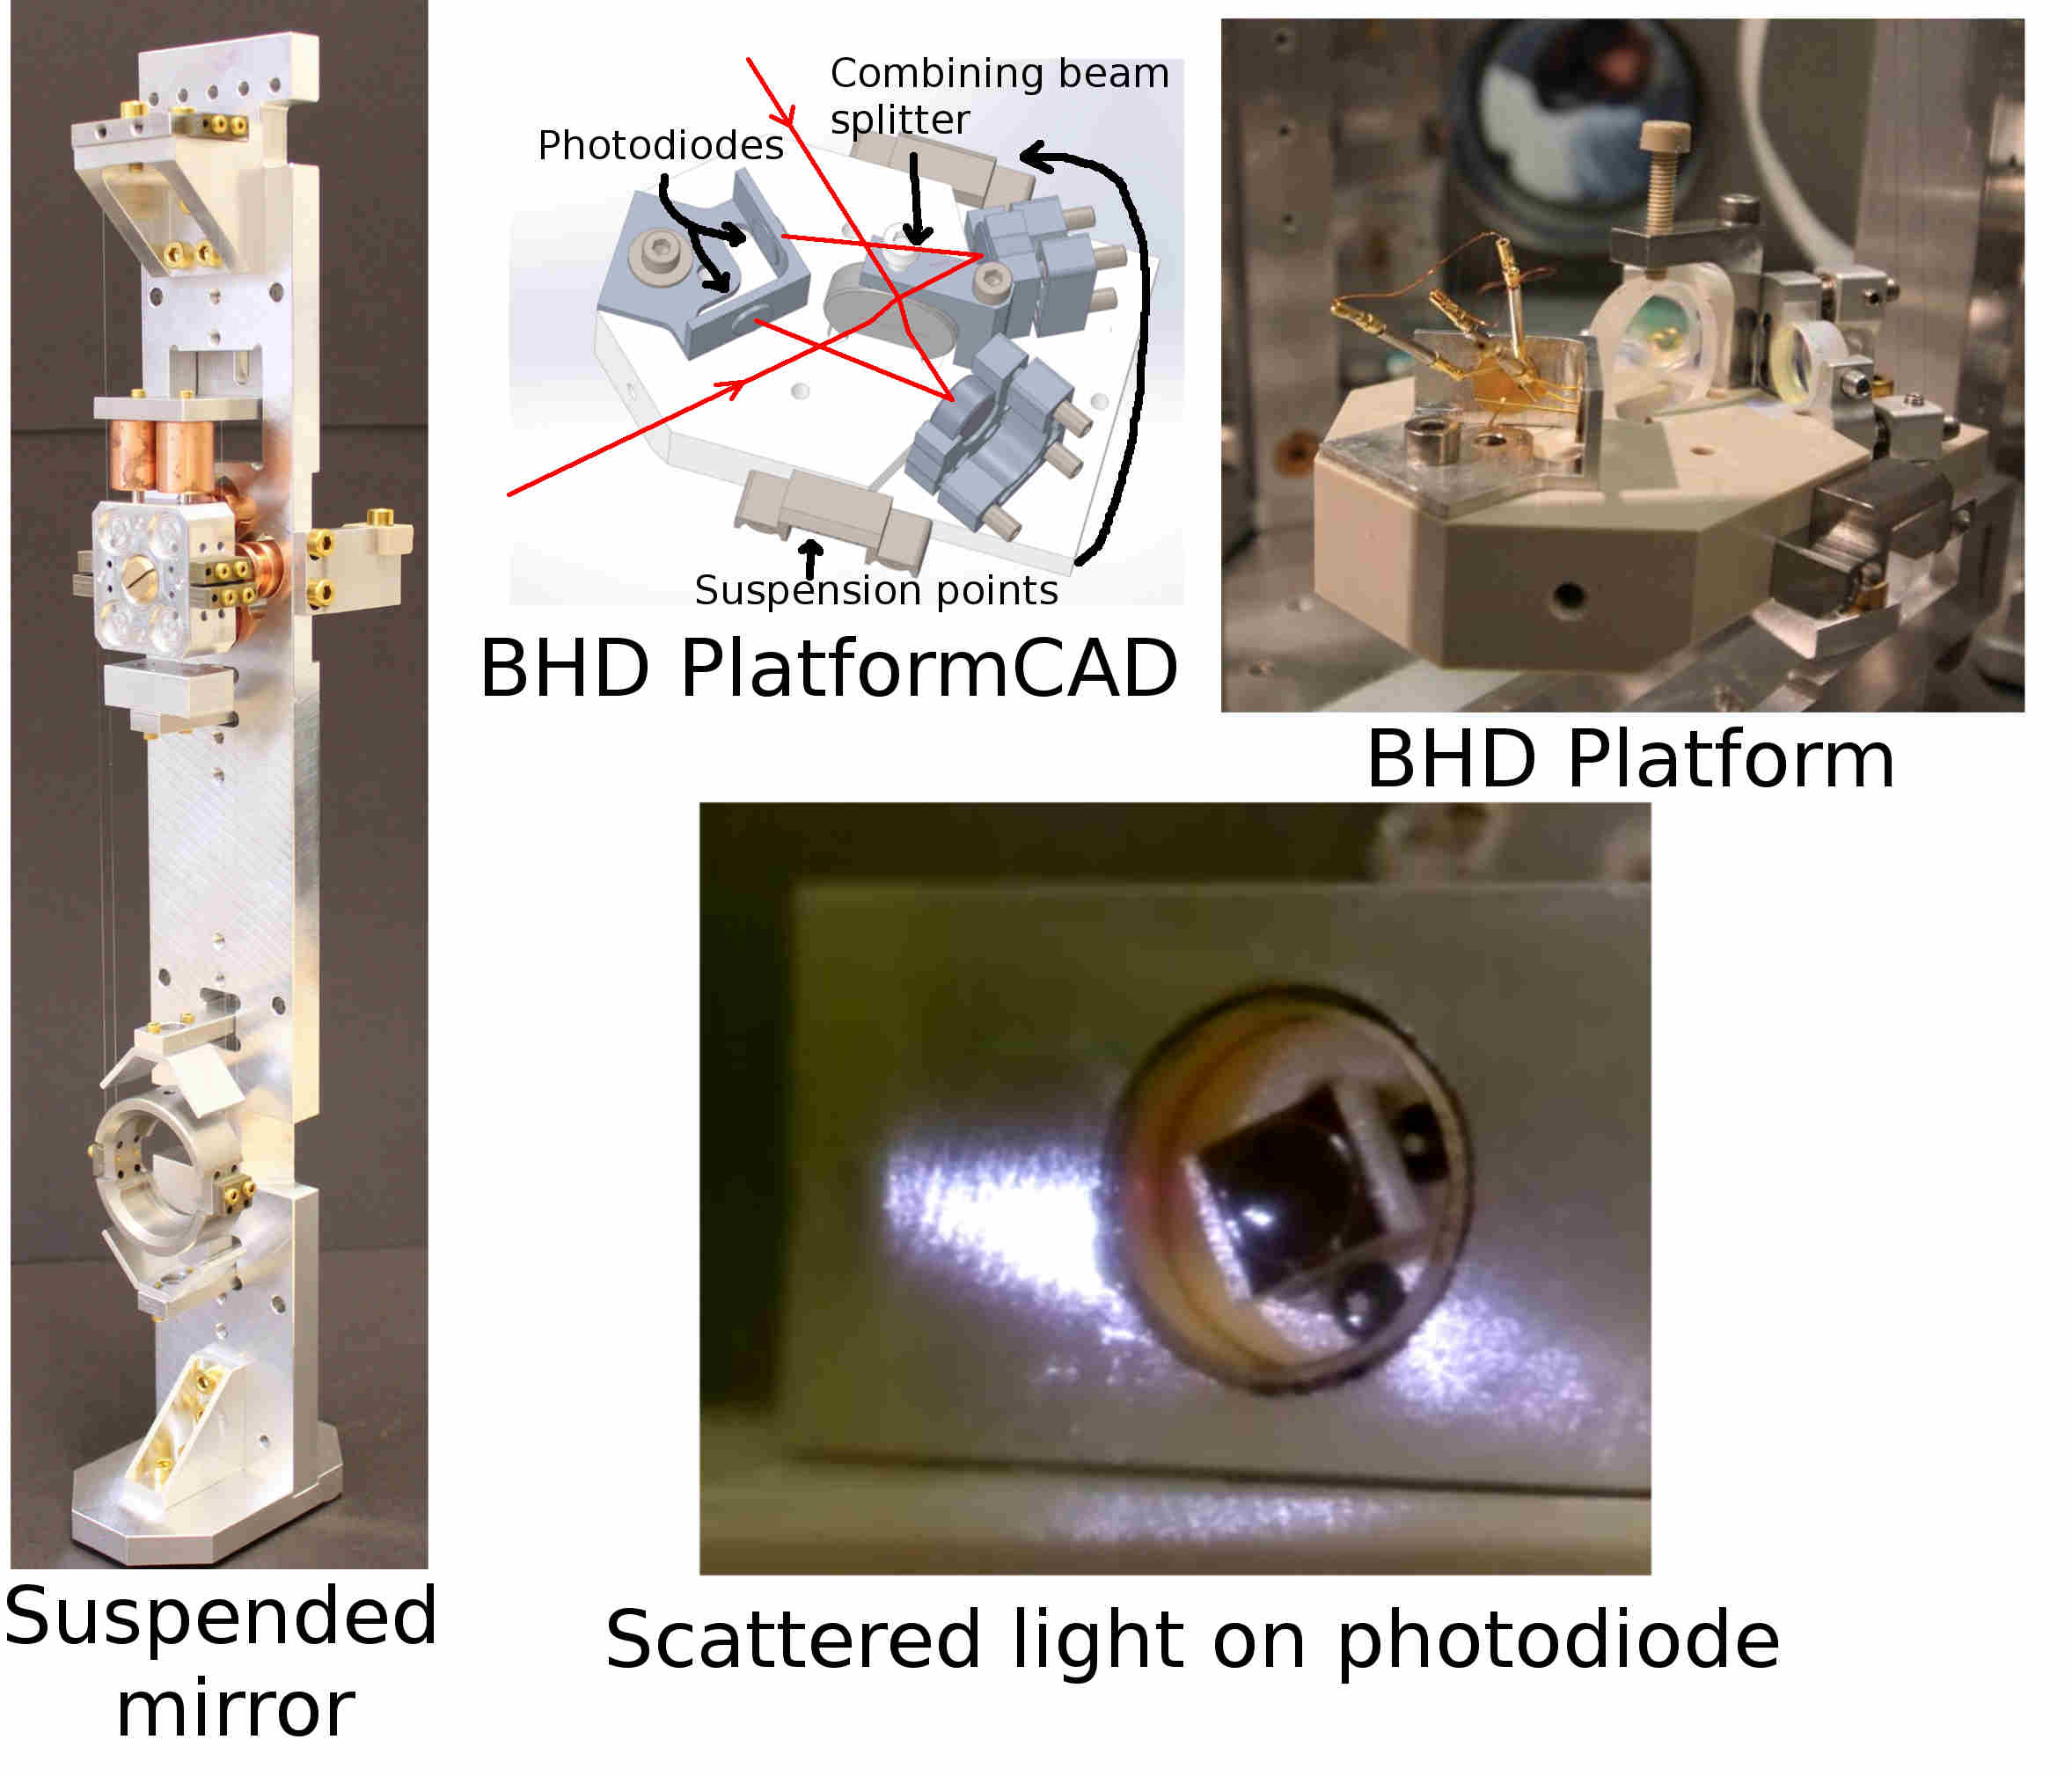
\includegraphics[width=1\linewidth]{Figures/MZ_chapter_in_vacuum_mz_apparatus}
	\caption{}
	\label{fig:mzchapterinvacuummzapparatus}
\end{figure}
\subsection{Calibration and Locking of the In-Vacuum Mach-Zehnder}
The differential arm length needed controlling below the suspension main resonance, ~ $\sim1$\,Hz as the optics moved on the order of one wavelength at these frequencies. Due to the design of the of the balanced homodyne readout, there are lots of suspension-related modes that couple to the longitudinal signal at around 30\,Hz. Additionally, the optical bench moved around a large amount due to poor seismic isolation. This meant that the differential arm length noise was at a similar level at $\sim30\,Hz$ as it was at $\sim1\,Hz$. 
\par
The suspended mirror was actuated on with a magnet+coil to lock the Mach-Zehnder arm length. The coil acted on a magnet glued to the bottom stage of the pendulum meaning that its strength fell as $1/f^2$ above the suspensions resonance. Thus, the coil would need to drive a large signal at $1$\,Hz, as well as one that was $~1000$ times greater at $\sim30$\,Hz. The magnet+coil strength was limited by geometry, e.g~ the size of the mirror, size of the magnet, size of the coil, amount of current that the coil could have etc., and so was not strong enough to do this. Therefore, the unity gain point needed a large gain at $\sim1$\,Hz while having a unity gain point limited to being below and $10$\,Hz by the suspension/coil driver actuator. To get the required gain, resonant gain filters were implemented in CDS, and to compensate for the phase problems these caused, phase compensation filters were made. \textcolor{red}{more detail?}
\par
The transfer function of the servo is shown in Figure \ref{fig:mzchapterflowdiagraminvacuumservo} and a sketch of the servo is shown in Figure \ref{fig:mzchapterflowdiagraminvacuumservo}. The servo consists of five logical blocks: the coil-driven suspended mirror, the `optical transfer function' that represents a change in differential arm length and the power of the recombined beam, the photodiode circuit, the analogue to digital/digital to analogue converters, and the digital filtering. The dewhitening filters were inverses of the whitening filter, and so they have no effect on the shape of the loop. As the transfer function of the suspension was simulated using the model developed in \ref{} and the digital filters just add shaping, to calibrate the loop, the conversion factors for the electronics and optics needed to be measured; this is summarised in table \ref{tab:MZ_chapter_servo_model}. 
\par
By injecting and measuring a signal across a `times one' block in the digital part of the servo, as the ratio of the two signals sizes gives the loop gain, the model's calibration was independently verified . This is shown in figure \ref{fig:mzchapterservotransferfunction}. This calibration ties up to within 0.1\,dB. Therefore, the unity gain point of the servo was at 5.5\,Hz with 15\si{\degree} of phase margin. 
\begin{table}
	\centering
	\begin{tabular}{|c|c|c|}
		\hline
		Component & Transfer function & unit \\
		\hline
		CDS DAC/ADC converters & 0.62 & mV/count\\
		Coil driver & 1.0 & mA/V \\
		Coil & 10 & mN/A \\
		Suspension & $H(f)$ & N/m\\ 
		Mach-Zehnder & 665000 & m/$\lambda$ \\
		Fringe to counts & 79000 & $\lambda$/count\\
		Digital filtering & $G(f)$ & count/count\\ 
		\hline
	\end{tabular}
\caption{Elements of the servo and their transfer functions. The suspension transfer function, $H(f)$, was obtained by simulation, the digital filter's transfer function is trivial, the coil's force per current was calculated using an existing script, the rest of the transfer functions were directly measured. These values were used to produce the servo model shown in Figure \ref{fig:mzchapterflowdiagraminvacuumservo}.}
\label{tab:MZ_chapter_servo_model}
\end{table} 
\begin{figure}
	\centering
	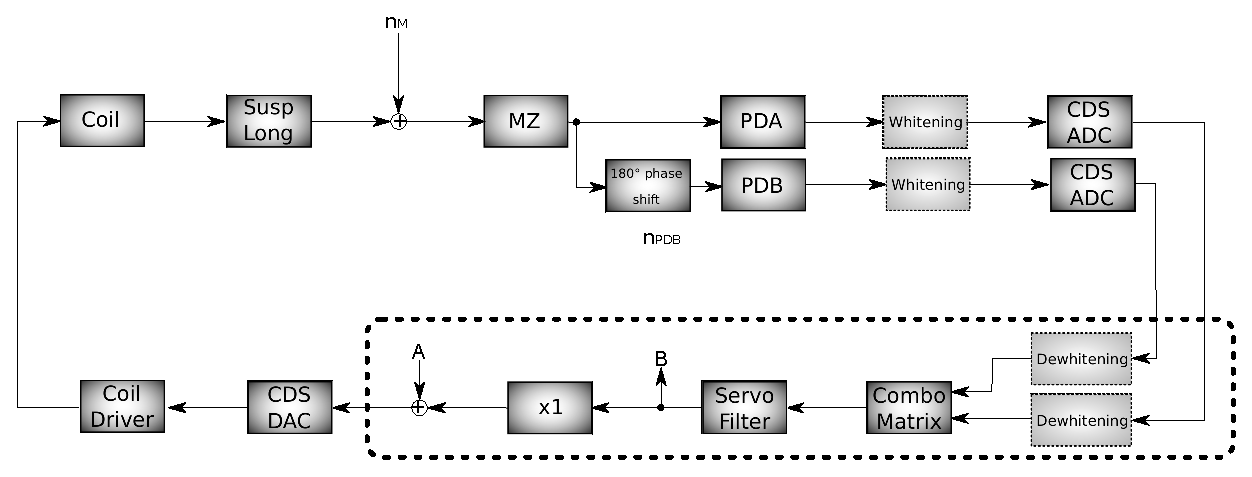
\includegraphics[width=1\linewidth]{Figures/MZ_chapter_flow_diagram_in_vacuum_servo}
	\caption{Flow diagram showing the each block of the servo used to lock the in-vacuum Mach-Zehnder. The digital part of the servo is shown in the dashed area. The injection points A and B were used to calibrate the servo (see Figure \ref{fig:mzchapterservotransferfunction} are around a times one block. The mirrors motion that the servo must correct for is represeted by the signal $n_M$. The information about the Mach-Zehnder differential arm length is encoded by two signals that are 180\si{\degree} out of phase. The whitening and dewhitening filters are paler as these do not affect the gain of the loop.}
	\label{fig:mzchapterflowdiagraminvacuumservo}
\end{figure}
\begin{figure}
	\centering
	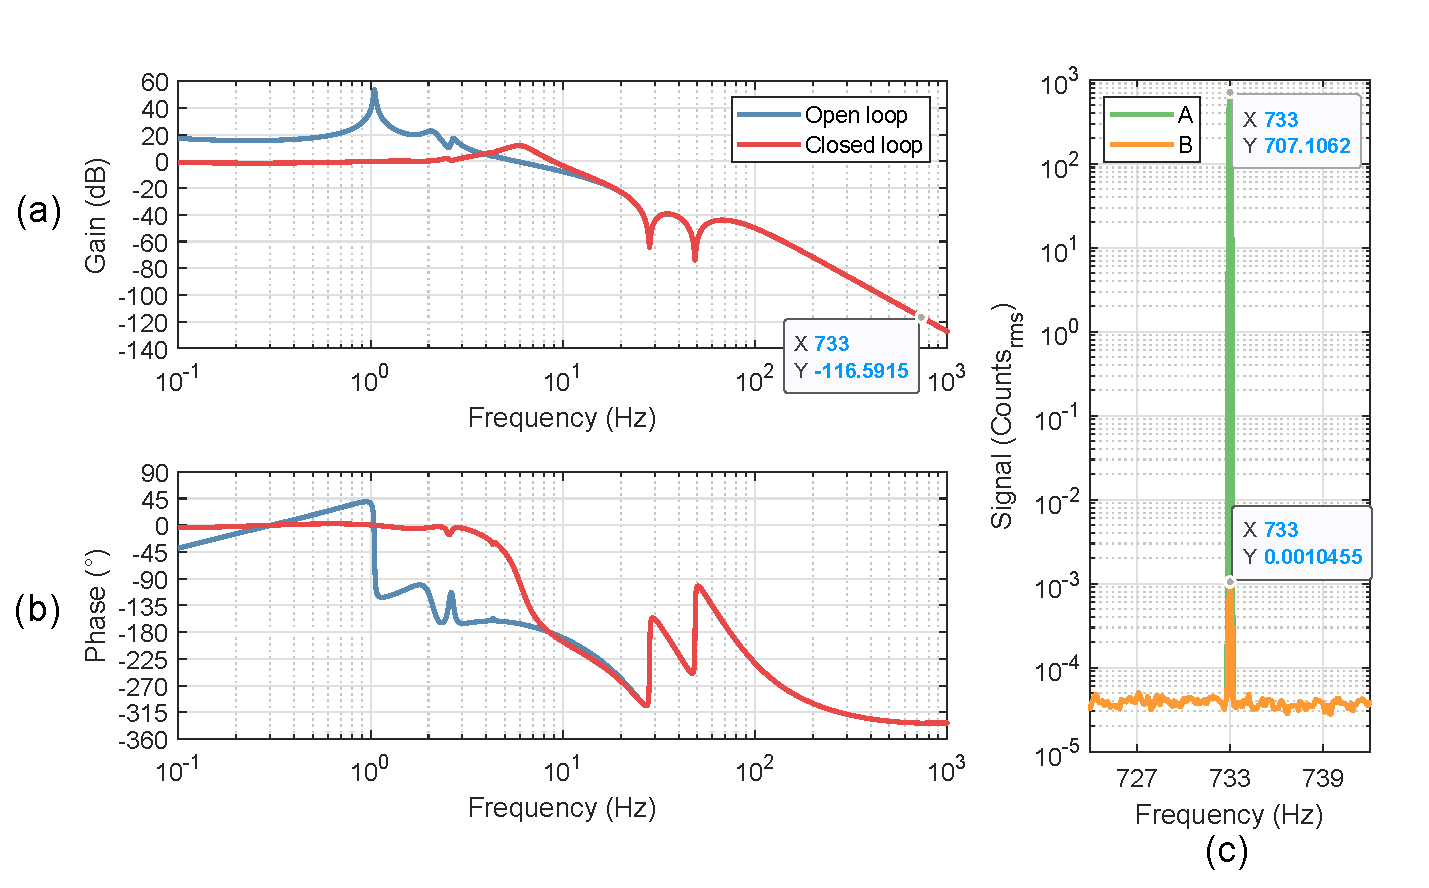
\includegraphics[width=1\linewidth]{Figures/MZ_chapter_servo_transfer_function_cali_combo}
	\caption{Panel (a) and Panel (b) is the Bode diagram of the Servo's open and closed loop transfer function. This was calibrated using the factors from \ref{tab:MZ_chapter_servo_model}. Panel (c) shows a measurement where a signal was injected at point A in the servo and measured at point B (see figure \ref{fig:mzchapterflowdiagraminvacuumservo}); these two points are separated by a times one block, and so the ratio of these signals represents the closed loop transfer function of the servo. These measurements are in agreement with the model to within 0.1\,dB.}
	\label{fig:mzchapterservotransferfunction}
\end{figure}
\subsection{Measurement of the Differential Arm Signal}
With the servo described in section \ref{}, the in-vacuum Mach-Zehnder was locked. The differential arm motion spectrum is shown in figure \ref{fig:mzchaptersuspendeddiffarm}. The curved steering mirrors used to guide the beam onto the photodiodes did not have an AR coating on their back face. This caused a large amount of scattered light. Scattered light generates a bilinear angle-to-intensity coupling. In an interferometer, this causes excess noise due to scattered light interfering with interferometers differential light mode. One of the great engineering achievements demonstrated at LIGO is the reduction of scattered light as this is currently a limiting source of noise at low frequencies. 
\begin{figure}
	\centering
	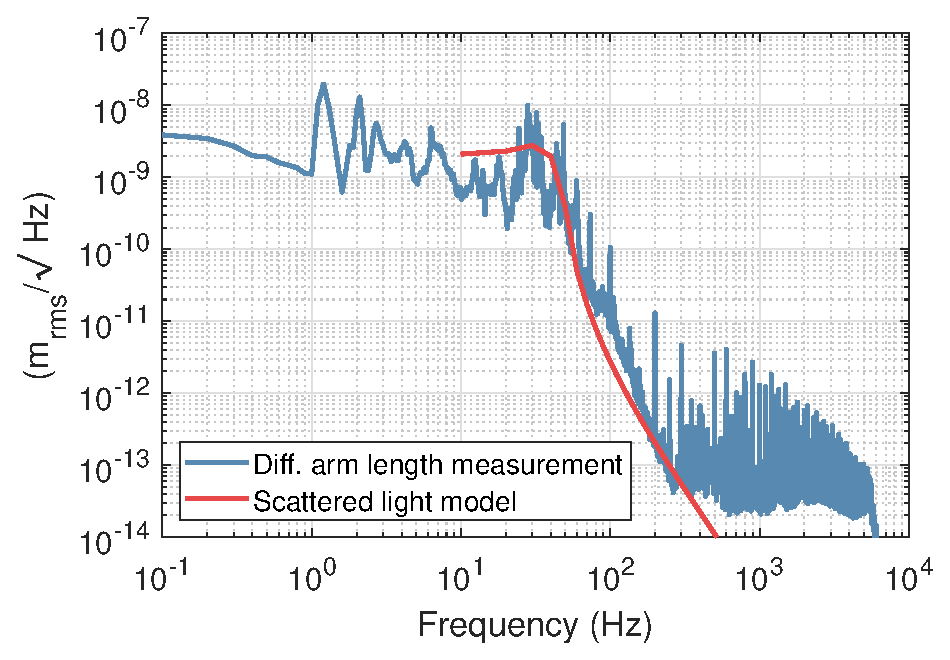
\includegraphics[width=1\linewidth]{Figures/MZ_chapter_suspended_diff_arm}
	\caption{Large amounts of scattering caused there to be a high amount of noise in the differential arm length signal's noise floor, this can be seen to limit the noise above $\sim200$\,Hz. The effect of the pendulums resonance at $\sim 1\,Hz$ was mostly removed by the servo but it can still be seen in the noise. Many suspension related peaks can be seen around 30\,Hz, these are due to the design of the BHD suspension. The $1/f^4$ slope is due to the suspension having two stages. For this measurement, shot noise would have been at $\sim 10^{-15}\,\rm{m}/\sqrt{\rm{Hz}}$.}
	\label{fig:mzchaptersuspendeddiffarm}
\end{figure}
\subsection{The Effect of Misalignment on the Size of a Signal in an Interferometer}
This apparatus can be used to verify that an angular misalignment, $\theta$, will cause the signal, $S$, to drop from its maximum value, $S_0$, as
\begin{equation}
S_{\rm{sig}} = S_0 e^{-\left( (\theta -\theta_0)/\theta_c\right)^2},
\label{eq:MZ_chapter_misalignment}
\end{equation}
where $\theta_c = \sqrt{2}\lambda_{\rm{EM}}/\pi w_0 $ is the characteristic angle of the a beam of waist $w_0$. The counts to angle was measured by applying the largest possible angle offset that CDS could provide and measuring the distance the beam moved, a few milimeter, over a distance of the order a metre. The beam's waist is know to be $\sim460\si{\micro\meter}$. A differential arm signal was generated and the resulting photodiode signal was measured for a range of angular misalignments. This result is shown in Figure \ref{fig:mzchaptermisalignmentplot}. To prevent noise at nearby frequencies from leaking into the measurement, a narrow frequency resolution was required (0.2\,Hz). Roughly 10 averages were made used to measure the signal size at each misalignment. The variance of these averages was large, this is represented by the error bars shown in figure \ref{fig:mzchaptermisalignmentplot}. A weighted non-linear least squares regression function (\textsc{Matlab}'s \texttt{nlinfit}) was used to fit the data to Equation \ref{eq:MZ_chapter_misalignment}, with each point weighted with $1/\rm{error}^2$. The resulting fit parameters were $S_0 = 6.9\pm0.3 \times10^{-3}$\,counts and $\theta_0 = 0.46\pm0.02\,\si{\milli\radian}$. The covariance between $S_0$ and $\theta_0$ was $\sigma_{S_0,\theta_c} = 2.4\times10^{-9}$ and the reduced $\chi^2$ statistic was 3.07.
\begin{figure}
	\centering
	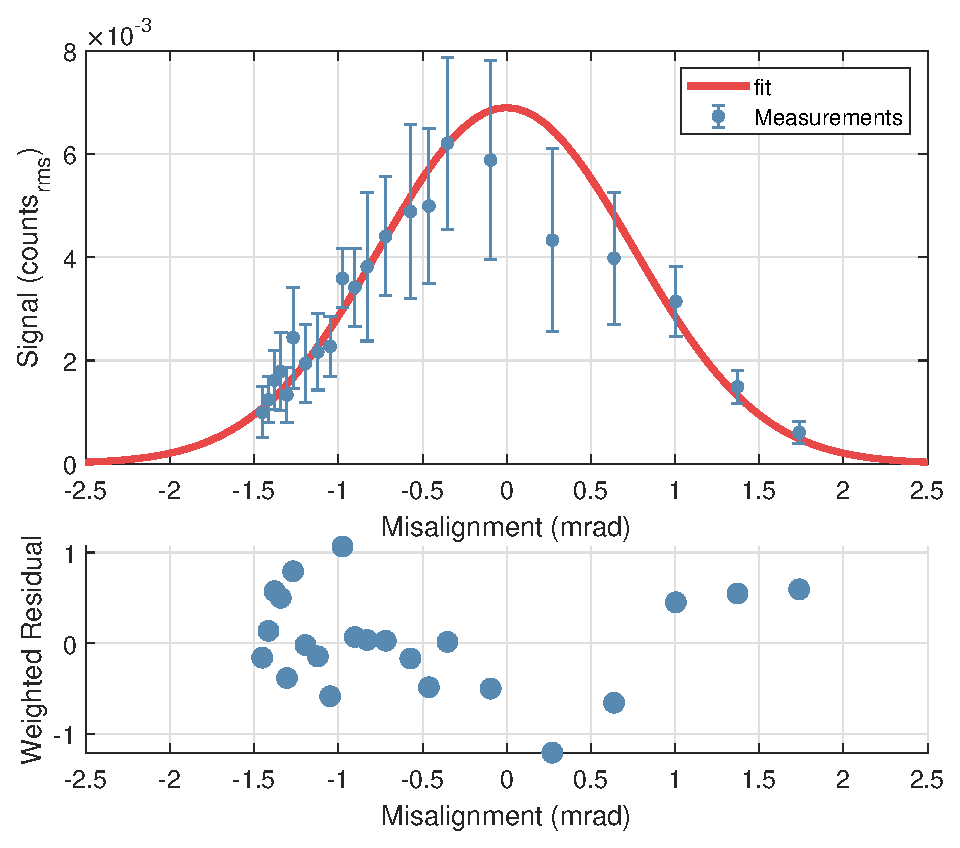
\includegraphics[width=1\linewidth]{Figures/MZ_chapter_misalignment_plot}
	\caption{Top panel: The in-vacuum Mach-Zehnder was misalignment. As the Mach-Zehnder was misaligned, there was less power in the HG00 mode. The decrease in power for a misalignment $\theta$ is  }
	\label{fig:mzchaptermisalignmentplot}
\end{figure}
\section{Conclusion}
A small, rigid mach zender was constructed to experimentally demonstrate the relationship between the local oscillators path length stability (see Equation \ref{eq:MZ_chapter_shot_noise_level}). This interferometer was calibrated and shot noise was measured. 

\chapter{In-vacuum experiments}
\section{Introduction}
why in vacuum. what measurements where made (need to think how these are interpreted still)
\section{apparatus}
\subsection{description of vacuum system}
\subsection{suspensions}
\subsection{photodiodes}
\subsection{measurement of table motion}
\section{control loop}
\subsection{transfer function simulation of suspension}
\subsection{analogue electronics}
\subsection{digital filering}
\section{Measurements}
\section{Discussion}
\chapter{Relevent Semiconductor and Photodiode Theory}
this chapter will give the essentials for understanding how a photon is turned into an electron by a photodiode. It will then talk about some details of how photodiodes are constructed. This will read as a `theory' chapter, but I will try to keep it short since all I need to do is explain what the 1/f noise is and what can be done to reduce it.
%\section{what is a semiconductor}
%\section{what is a diode}
%\section{what is a PIN junction}
%\section{what is a photodiode and basic properties of them}
%\section{Possible materials for photodiodes}
%\section{Dark current}
%\section{1/f noise sources in semiconductors}
%\section{growth techniques for photodiodes and why its important}

\chapter{Characterisation of InGaAs Photodiodes}
should this be an appendix?
\chapter{Characterisation of Extended InGaAs Photodiodes}
\graphicspath{ {paper/} }
\section{Introduction and requirements}
\subsection{Wavelength choice}
\subsection{Semiconductor choice}
\subsection{Quantum efficiency}
\subsection{linearity}
\subsection{Quantum noise from modulation demodulation emphasis}
\subsection{low levels of dark noise (1/f)}
\subsection{size of diode}
\section{`Bare minimum' Photodiode Theory}
\subsection{what is a semiconductor}
\subsection{what is a diode}
\subsection{what is a PIN junction}
\subsection{what is a photodiode and basic properties of them}
\subsection{Possible materials for photodiodes}
\subsection{Dark current}
\subsection{1/f noise sources in semiconductors}
\subsection{growth techniques for photodiodes and why its important}
\section{List of experiments done on extended InGaAs}
to test the requirements above...
\subsection{dark noise measurements}
\subsubsection{dark noise as function of bias}
\subsubsection{dark noise as function of temperature}
\subsection{Light based tests}
\subsubsection{lock-in style measurements to measure QE change}
\subsubsection{DC style measurements to measure QE change}
\subsubsection{Shot noise measurement to validate QE change}
\subsubsection{lock in style measurement to test linearity}
\subsection{List of experiments done on Hammamatsu P5968-100 InSb}
Promising data sheet, showed high QE and linearity. This is still to be done
\section{Apparatus for measurements in each subsection above}
\section{Discussion of the results for each subsubsection above}
\section{Conclusion}
\section{Current write up in paper form}
\paragraph{}
Below is currently just the paper I was working on. More detail will go in, as well as additional measurements + results which I haven't written up. This is here a place holder for now.
\section{abstract}
High quantum efficiency, low noise photodiodes are a fundamental part of the readout of ground based gravitational wave detectors. The 3rd generation of these detectors may be operated with either a 1550\,nm or around 2000\,\SIunits{\nano\metre} wavelength laser as a consequence for the potential to develop cryogenic compatible coatings and test masses for these wavelengths. The current InGaAs photodiodes which are used for the readout of gravitational wave detectors would not be compatible with a 2\,\SIunits{\micro\metre} laser. Extended InGaAs is a potential material that could be used for these photodiodes and can be purchased with a variety of cut-off wavelengths up to \SIunits{2.6}{\,\micro\metre}. In this paper, several off-the-shelf extended InGaAs photodiodes with different cut-off wavelengths were characterised. The dark noise, linearity and quantum efficiency of these photodiodes was investigated to see if there were optimal operating conditions which would provide a high enough quantum efficiency while still being low enough noise as to not limit the noise performance of the interferometer. It was found that the photodiodes tested do not meet the requirements of a 3rd generation gravitational wave detector. Longer cut-off wavelength photodiodes tended to perform more poorly than photodiodes with a shorter cut off wavelength in terms of noise performance and linearity, although this varies between manufacturer. While under a usable reverse bias voltage the highest quantum efficiency measured was 70\%. While its possible to achieve higher quantum efficiencies the noise of the photo-current will not be limited to shot noise in the detection frequency band of a gravitational wave detector, $\sim$100\,Hz, due to large amounts of $1/f$ noise. This due to it being technically challenging to fabricate extended InGaAs which is thick enough to have a high quantum efficiency while also having a low amount of defects.
\section{Introduction}
Einstein predicted the existence of gravitational waves, and since 2015 a catalogue of detections has been made \cite{Collaboration2018}. As well as being a test of general relativity, the detection of gravitational waves has ushered a new era of astronomy, giving us the ability to directly observe astrophysical objects such as binary black holes and binary neutron stars \cite{Abbott2017a}. With a global network of kilometre scale interferometers, multi-messenger astronomy has already yielded exciting new results. Measurements of gravitational waves emitting the from  merging of binary neutron stars has tested the equivalence principle \cite{Abbott2017c}, given us bounds on the speed of gravity and allowed us to test the value of the Hubble constant \cite{Abbott2017d}, as well as giving us insights into the origin of heavy elements \cite{Kasen2017}.
%\paragraph{}
%As the current generation of detectors are reaching their design sensitivity, work is beginning on the next generation of detectors. Once LIGO has reached its design sensitivity, it will be dominated by the coating thermal noise in its detection band (around 100\,Hz)\cite{a+curve}. This noise source is due to the Brownian motion of the molecules in the coating which creates the mirror surface. Due to the thermal noise of the optical coatings being a limiting source of noise \cite{InstrumentWhitePaper2018}, proposed future gravitational wave detectors such as the Einstein Telescope \cite{Punturo2010} and LIGO Cosmic Explorer \cite{Abbott2017e} will use cryogenically cooled mirrors. Since the current coatings do not improve much when cooled, a new coating will need to be developed. The coatings for these mirrors will be compatible with a 2\,\SIunits{\micro\meter} or a 1550\,nm wavelength laser, instead of a 1064\,nm laser that current gravitational wave detectors use. Changing the wavelength of the laser to 2\,\SIunits{\micro\meter} means that the current InGaAs photodiodes used will not be suitable since typical InGaAs photodiodes are not sensitive to this wavelength.
\paragraph{} %Bryans paragraph
As the current generation of gravitational wave detectors reach their design sensitivity, researchers are looking to the future and how to improve the sensitivity of the next generation of detectors. Once at design sensitivity, the noise floor of LIGO will be limited by mirror coating thermal noise (Brownian motion of the molecules in the mirror surface) in the detection band (around 100 Hz)\cite{a+curve}. Since these thermally driven fluctuations are a limiting source of noise \cite{InstrumentWhitePaper2018}, proposed future gravitational wave detectors such as the Einstein Telescope \cite{Punturo2010} and LIGO Cosmic Explorer \cite{Abbott2017e} will use cryogenically cooled mirrors. To take full advantage of this approach will require the development of new cryogenically optimised coatings and switching the operating laser wavelength to \SIunits{1550}{\,nm} or around 2000\,\SIunits{\nano\metre}, instead of the \SIunits{1064}{\,nm} wavelength used in current gravitational wave detectors. Changing the wavelength of the laser to 2\,\SIunits{\micro\metre} means that the current InGaAs photodiodes used in the readout of gravitational wave detectors will not be suitable since typical InGaAs photodiodes are not sensitive to 2\,\SIunits{\micro\metre} light.
\paragraph{}
Current gravitational wave detectors operate in the 1-10\,mW range at the output \cite{Prijatelj2012} to ensure that the junk light from other modes is a small portion of the total signal. Thus, any new photodiode should be able to produce $\sim$10\,mA of photo-current. The photodiodes used in the readout of a gravitational wave interferometer should have a quantum efficiency of more than 99\%. The reason for having such a high quantum efficiency requirement is that to achieve the baseline level of $\sim$10\,dB of squeezed light that future gravitational wave detectors will use, losses in the interferometer have to be extremely low as losses degrade the amount of squeezing achieved. Photodiodes for gravitational wave detectors should have low $1/f$ dark noise so that they are not limited in the detection band by electronic noise. Third generation ground based gravitational wave detectors will be quantum noise limited down to about 10\,Hz \cite{Harry2010}, so the $1/f$ noise must be below the shot noise of the photo-current above this frequency. The $1/f$ noise could potentially be reduced by using external modulation, however the shot noise would increase if the mixing of the modulation and demodulation waveforms was not time independent \cite{Meers1991}, which limits the choice of waveforms. A modulation-demodulation scheme such a external modulation with a $\pi$ square wave has been considered, but this comes with a significant technical difficulty in creating a suitable EOM driver, and remains to be proven \cite{Meers1991}. Even if the EOM was driven with a good enough square wave, the use of squeezing means that this approach would still not be sufficient as adding higher harmonics boosts the signal rather than reduces noise. In other words, the noise improvement from squeezing would be lost.
\paragraph{}
If the wavelength that gravitational wave detectors are operated at changes to 2\,\SIunits{\micro\meter} then extended InGaAs would be a candidate material for the readout photodiodes. Extended InGaAs has more than the usual 53\% indium found in conventional InGaAs diodes, as this reduces the size of the bandgap thus and increases the cut-off wavelength. Increasing the reverse bias voltage increases the quantum efficiency of extended InGaAs photodiodes, and data sheets for these devices show that there is a relationship between quantum efficiency and temperature. Several extended InGaAs photodiodes were tested to see if there was a combination of bias voltage and temperature that would improve the quantum efficiency whilst keeping the $1/f$ noise low. It was found that noise at temperatures between 0\,\SIunits{\degree C} and room temperature was almost entirely dependant on reverse bias voltage and did not improve as the device was cooled. It was found that to get adequate noise performance, the diodes needed to be used at a reverse bias voltage that meant their quantum efficiency was far below the requirement of  third generation gravitational wave detector. This $1/f$ noise and quantum efficiency problem has limited previous squeezing experiments using 2\,\SIunits{\micro\meter} lasers \cite{Mansell2018a}. For instance, the FD10D from Thorlabs was measured to have a quantum efficiency of 82\% at \SIunits{1550}{\,nm} when used at its full rated reverse bias, and at this bias the $1/f$ noise only became less than a typical shot noise above \SIunits{1}{\,kHz}.  When asked about the possibility of procuring a diode that meets the requirements set out above, the responses from manufacturers ranged from saying such a diode is impossible to construct to saying that money is the main obstacle.
\section{PIN InGaAs Photodiodes}
PIN photodiodes use a positive-intrinsic-negative semiconductor structure to create a device that when light of sufficient energy, energy greater than the band gap of the semiconductor, is incident on it an electron-hole pair is produced. Within the P region there is an excess of holes and within the N region there is an excess of electrons. This region is called the depletion region. The intrinsic semiconductor is used to make the depletion region of the photodiode wider. Due to the electric field between the P and N regions, electron-hole pairs that are produced in the depletion region due to an incident photon results in electrons moving towards the N-type semiconductor and holes drifting towards the P-type semiconductor, thus creating a current. By applying a reverse bias, the depletion region is widened resulting in the conversion of light to current being more efficient. The ratio of total photons incident on the photodiode to photons which produce electrons-hole pairs is called quantum efficiency.
\paragraph{}
Photodiodes produce a dark current $I_d$ which depends on the reverse bias. The dominant source of dark current depends on the regime of reverse bias that the diode is under and can be separated into three sources: diffusion current $I_{\mathrm{diff}}$; generation-recombination current $I_{\mathrm{GR}}$ and quantum tunnelling current $I_{\mathrm{tun}}$ \cite{Forrest1981},
\begin{equation}
I_d = I_{\mathrm{tun}} + I_{\mathrm{diff}} + I_{\mathrm{GR}}.
\end{equation}
$I_{\mathrm{tun}}$ arises due to electrons being able to tunnel across the band gap, similar to the breakdown voltage of a diode. $I_{\mathrm{diff}}$ arises due to the diffusion of minority carriers into the intrinsic region. $I_{\mathrm{GR}}$ is due to the generation and recombination of electron hole pairs in the intrinsic region, and the random nature of the generation and recombination of electron hole pairs is the source of $1/f$ noise \cite{Seifert2010}. This noise is sometimes referred to as Shockley-Read-Hall (SRH) noise (or more generally for $1/f$ noise with a different physical origin as random telegraph or popcorn noise). Electrons and holes enter what are known as trap states, states which ideally would not exist, and the amount of time spent there before leaving and recombining with electrons and holes is random. These states can arise due to lattice mismatching. The spectrum of one trap causing generation-recombination of electrons and holes is a Lorentzian which when many traps are near each other can look like a $1/f$ spectrum \cite{Klumperink}\cite{Machlup1954}\cite{Hooge1981}. This theory also allows for noise spectra which are nearly $1/f$, or have bends in them.
%\begin{equation}
%S(\omega) = \frac{1}{\pi}\cfrac{\sigma\tau}{(\sigma+\tau)^2}\cfrac{\cfrac{1}{\sigma}+\cfrac{1}{\tau}}{\omega^2 + \left(\cfrac{1}{\sigma}+\cfrac{1}{\tau}\right)^2}
%\label{eq:lorentzian}
%\end{equation}
%\begin{figure}
%	\centering
%	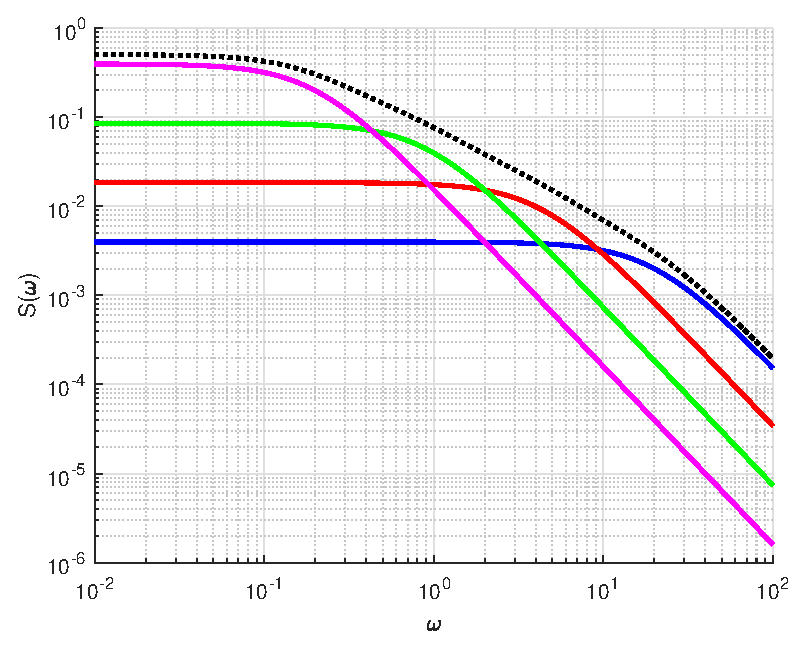
\includegraphics[width=0.7\linewidth]{other_figures/McWortersModel}
%	\caption{By combining several Lorentzian spectra, $1/f$ noise is produced. The dashed line shows the sum of the coloured lines, which has a region where the spectrum is $1/f$. The coloured lines are determined by equation \ref{eq:lorentzian}, with $\sigma = \tau$ and computed for $\sigma \in \{0.1,0.46,2.15,10\} $.}
%	\label{fig:mcworter}
%\end{figure}
\section{Technical Problems In Creating Extended InGaAs Photodiodes.}
InGaAs is a widely used semiconductor for fabricating photodiodes. Typically they are sensitive up to wavelengths around 1550\,nm, however longer wavelength sensitivity can be achieved by increasing the amount of indium doping. These photodiodes are often called `extended' and can be sensitive for wavelengths up to 2.6\,\SIunits{\micro \metre}. One of the main issues faced when creating an extended InGaAs photodiode is the lattice mismatch between the InGaAs and the InP substrate on which its grown. Lattice mismatching can arise due to a strained crystal structure, and since the extra indium in an extended InGaAs photodiode causes this \cite{Gendry1992} it is hard to fabricate a low noise extended InGaAs photodiode \cite{Martinelli1988}. Above 53\% indium, a buffer layer of InGaAs with less indium in between the absorbing layer and the substrate can be used to mitigate the lattice mismatch slightly, but the dislocations still give rise to trap states which cause the generation and recombination of charge carriers \cite{Zimmermann2003}. Lattice mismatching is the source of the large amounts of dark current found in extended InGaAs as well as the $1/f$ noise.
\paragraph{}
Creating a photodiode with the quantum efficiency requirements of third generation gravitational wave detectors is difficult to achieve as the lattice mismatch makes it hard to make the photodiode thick enough since the critical thickness of extended InGaAs is only hundreds of angstroms \cite{Gendry1992}. The parameters that affect the internal quantum efficiency are the absorption coefficient of the extended InGaAs and the amount of the extended InGaAs material the light must travel through. For InGaAs that is sensitive to 2\,\SIunits{\micro\metre} the absorption coefficient, $\alpha$, is approximately $10^4$\,cm$^{-1}$ \cite{Alam2007}. To estimate the required thickness, $x$, of InGaAs to achieve 99\% quantum efficiency, we can use the Beer-Lambert law, $\frac{I_x}{I_0} = e^{-\alpha x}\label{eq:absorbtion}$ to find that $x = 4.6\,\micro\metre$. Although this is just a rough calculation, it does give one an idea of how thick the material needs to be. This assumes all the photons absorbed make it out of the junction as electrons/holes, which may not be the case as without a high enough bias the electrons will fail make it out of the junction before recombining with a hole. 
\paragraph{}
To ensure a low amount of strain, the layer of InGaAs could only be about 100\,nm thick between the InP and the InGaAs layer if the diode were to be constructed in the typical PIN arrangement. Above this thickness, dislocations due to the InGaAs not being lattice matched to the InP are a problem. The thicker the InGaAs layer is, the more strain relief is required between the InP substrate and the InGaAs layer. The more strained the InGaAs is, the more dislocations there will be which will lead to more $1/f$ noise and dark current. The critical thickness is the thickness above which the semiconductors quality degrades significantly, and the higher the ratio of indium to gallium, the thinner this critical thickness becomes \cite{Anan1992}. Putting 100\SIunits{\,\nano\metre} into the Beer-Lambert law gives an internal quantum efficiency of about 10\% which is far below the requirements for GW detectors. The amount of threading dislocations contained within an InGaAs photodiode can be reduced by orders of magnitude with careful choice of growth conditions and design of the layers in the photodiode \cite{Chen2018}\cite{Zimmermann2003}.
\paragraph{}
Another design challenge arises because InGaAs is not a good conductor of heat so a thicker amount of InGaAs can lead to lower power handling before the diode is thermally destroyed\cite{Li2004}. Once the internal quantum efficiency problem has been solved, an anti reflection coating would need to be developed. InGaAs that is optimised for 2\,\SIunits{\micro\metre} has a refractive index, $n$, of approximately $3.6$ \cite{Alam2007}. Assuming a single quarter-wave layer was to be applied, the film would need a refractive index that was $n_f = \sqrt{3.6}$ and be 600\,\SIunits{\nano\meter} thick. The idea of using this anti reflective coating as a passivation layer is presented in \cite{L_pez_2007}. 
\section{Apparatus}
When designing a photodiodediode circuit, the parameter space includes (but isn't limited too): reverse bias voltage used, size of the diode, temperature of the diode, cut-off wavelength and vendor. Each of these parameters could effect the noise performance and quantum efficiency of the photodiode, so experiments were designed to gain insights into where a diode which is suitable for a third generation gravitational wave detector readout scheme resides inside this space. The reverse bias  changes the amount of 1/f dark noise of the photodiode. Therefore, measuring when the reverse bias would cause the dark noise to become larger than the shot noise for a typical light level in a gravitational wave detector was investigated. Different levels of Indium doping effects the amount of strain that the semiconductor experiences, so the dark noise of devices with different cut-off wavelengths was investigated. The size of the diode also can effect the amount of dark noise, since there is more material to generate the noise, so devices of different sizes were characterised. If certain vendors had better manufacturing processes, that would also affect the noise. The dependence of dark $1/f$ noise on temperature was investigated to see if this $1/f$ dark noise can be reduced if the temperature is decreased from room temperature to 0\,\SIunits{\degree C}. To gain insights into how each of the variables mentioned affect the dark noise and to have a workable size of the parameter space to explore, the diodes shown in table \ref{tab:photodoides} were tested. To help identify the mechanism by which the dark noise is created in these kinds of diodes, the forward current voltage curve was measured and the ideality factor was determined. 
\paragraph{}
The requirements for an experimental characterisation of the chosen photodiodes are a) a dark box within which the experiment may be conducted, b) availability of a variable, low-noise bias voltage and c) a means by which the temperature of the device under test can be varied and controlled. Further, a suitably low-noise amplifier is required to monitor the photo-current and convert it to a voltage. To measure the dark current produced by multiple different photodiodes under different reverse bias voltages and easily obtainable temperatures, a dark box containing a Peltier module was constructed. The photodiode was held in place against a piece of aluminium that was also in contact with the Peltier and an LM35 temperature sensor was used to measure the temperature of the aluminium. The dark current of the photodiodes was expected to be of the order nanoamps so a 1\,\SIunits{\mega\ohm} resistor was used in the transimpedance amplifier. Due to this choice of resistor a TL071 op amp was used, as shown in Figure \ref{fig:tl071}. The bias voltage was provided by a LM7815 voltage regulator and since not much current was being drawn a variable resistor was used to set the bias voltage. A 1000\SIunits{\micro F} electrolytic capacitor was used to reduce the bias voltage noise. The low noise fixed bias circuit shown in figure \ref{fig:darknoisetestbox2} was constructed to verify that the more flexible swappable photodiode dark noise circuit would work.
\begin{table}
	\centering
	\begin{tabular}{| c | c | c | c |}
		\hline
		Part Name & Vendor & Cut-off Wavelength & diameter  \\ \hline
		IG19x1000S4i4 & Laser Components & 1.9\,\SIunits{\micro\metre} & 1\,mm \\ 
		IG22x1000S4i4 & Laser Components & 2.2\,\SIunits{\micro\metre} & 1\,mm \\ 
		IG24x500S4i4 & Laser Components & 2.4\,\SIunits{\micro\metre} & 0.5\,mm \\ 
		IG26x500S4i4 & Laser Components & 2.6\,\SIunits{\micro\metre} & 0.5\,mm \\ 
		FD01D & Thorlabs & 2.6\,\SIunits{\micro\metre} & 1\,mm \\ 
		G12183-020K & Hamamatsu & 1.9\,\SIunits{\micro\metre} & 2\,mm \\ \hline
	\end{tabular}
\caption{Extended InGaAs photodiodes used in the experiment.}
\label{tab:photodoides}
\end{table}
\paragraph{}
The quantum efficiency of the photodiode was measured as the reverse bias was changed. The reverse bias voltage affects the quantum efficiency since it affects the amount of time charge carriers spend in the depletion region, a lower bias allows more time for electrons and holes to recombine thus lowering the quantum efficiency. By measuring the photocurrent as the bias was increased for a fixed light power, the relative change in quantum efficiency as a function of reverse bias can be investigated. This can be verified as a genuine increase in quantum efficiency, and not a multi-charge carrier process, if the noise of the photocurrent can be stabilised to shot noise. Measuring the DC photocurrent and the amplitude of a modulation of the laser intensity as a function of reverse bias and light power allows for the region in which the photocurrent was linear to be determined. This requires an amplitude stabilised laser with a wavelength which the diodes in table \ref{tab:photodoides} are sensitive to and a variable bias voltage circuit for testing the extended InGaAs photodiodes under different biases.
\begin{figure}
\centering
%\begin{subfigure}{0.5\textwidth}
	\centering
	\includegraphics[width=0.5\linewidth]{Dark_noise_test_box_1}
%	\label{fig:tl071_circuit}
%\end{subfigure}%
%\begin{subfigure}{0.5\textwidth}
%	\centering
%	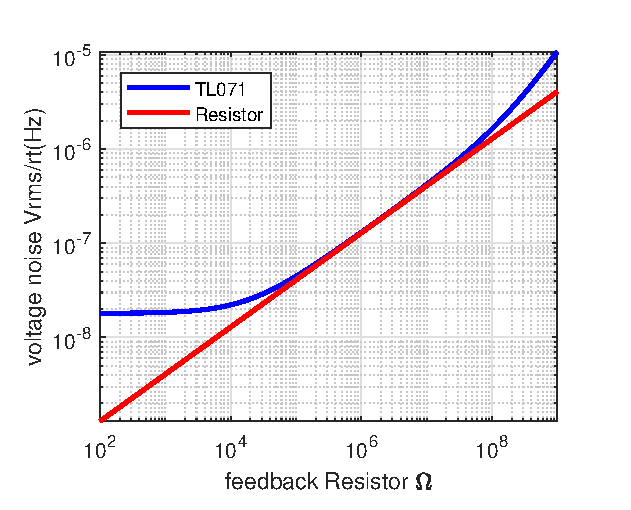
\includegraphics[width=1\linewidth]{tl071_tia_voltage_noise}
%	\caption{}
%	\label{fig:tl071_noise}
%\end{subfigure}
\caption{The transimpedance amplifier used to measure the dark noise of a variety of photodiodes. For large feedback resistors (R2 in the circuit above), a JFET style OP amp such as the TL071 performs better since these have low current noise (e.g. see \cite{AD797} for a description of noise sources in OP amp circuits). In this application, the TL071 is optimised for between 100\,\SIunits{\kilo\ohm} to 10\,\SIunits{\mega\ohm}.}
\label{fig:tl071}
\end{figure}
\paragraph{}
To measure the relative quantum efficiency and linearity of photodiodes at light powers up to 20\,mW, a 1500\,nm wavelength laser (PPCL300 from Pure Photonics) was used. The transimpedance amplifier shown in Figure \ref{fig:ad797pdtester} was built to test the photodiodes under different bias voltages. A low passed bench top power supply was used to provide the DC bias voltage. Without filtering it was found that the noise of the power supply was the limiting source of noise when there was laser light on the extended InGaAs photodiodes, as the impedance of the photodiodes decreased when light was on the photodiode. To prove that the increase in photo-current was due to an increase in the reverse bias, the shot noise of the photo-current was measured. To do this an amplitude stabilised laser was required. A none extended Excelitas InGaAs photodiode (C30641GH) was used for this and it was assumed this diode behaved well (this range of photodiodes is widely used in LIGO). The apparatus is shown in Figure \ref{fig:testsetup}. The half waveplate and polarising beam splitter allow for different DC light level to be controlled. Since at least 50\% of the light was always directed onto the photodiode used for the amplitude stabilisation, the light was shot noise limited for all accessible light powers. The lens was used to adjust the spot size. To make the measurements, an spectrum analyser was used. 
\begin{figure}
	\centering
	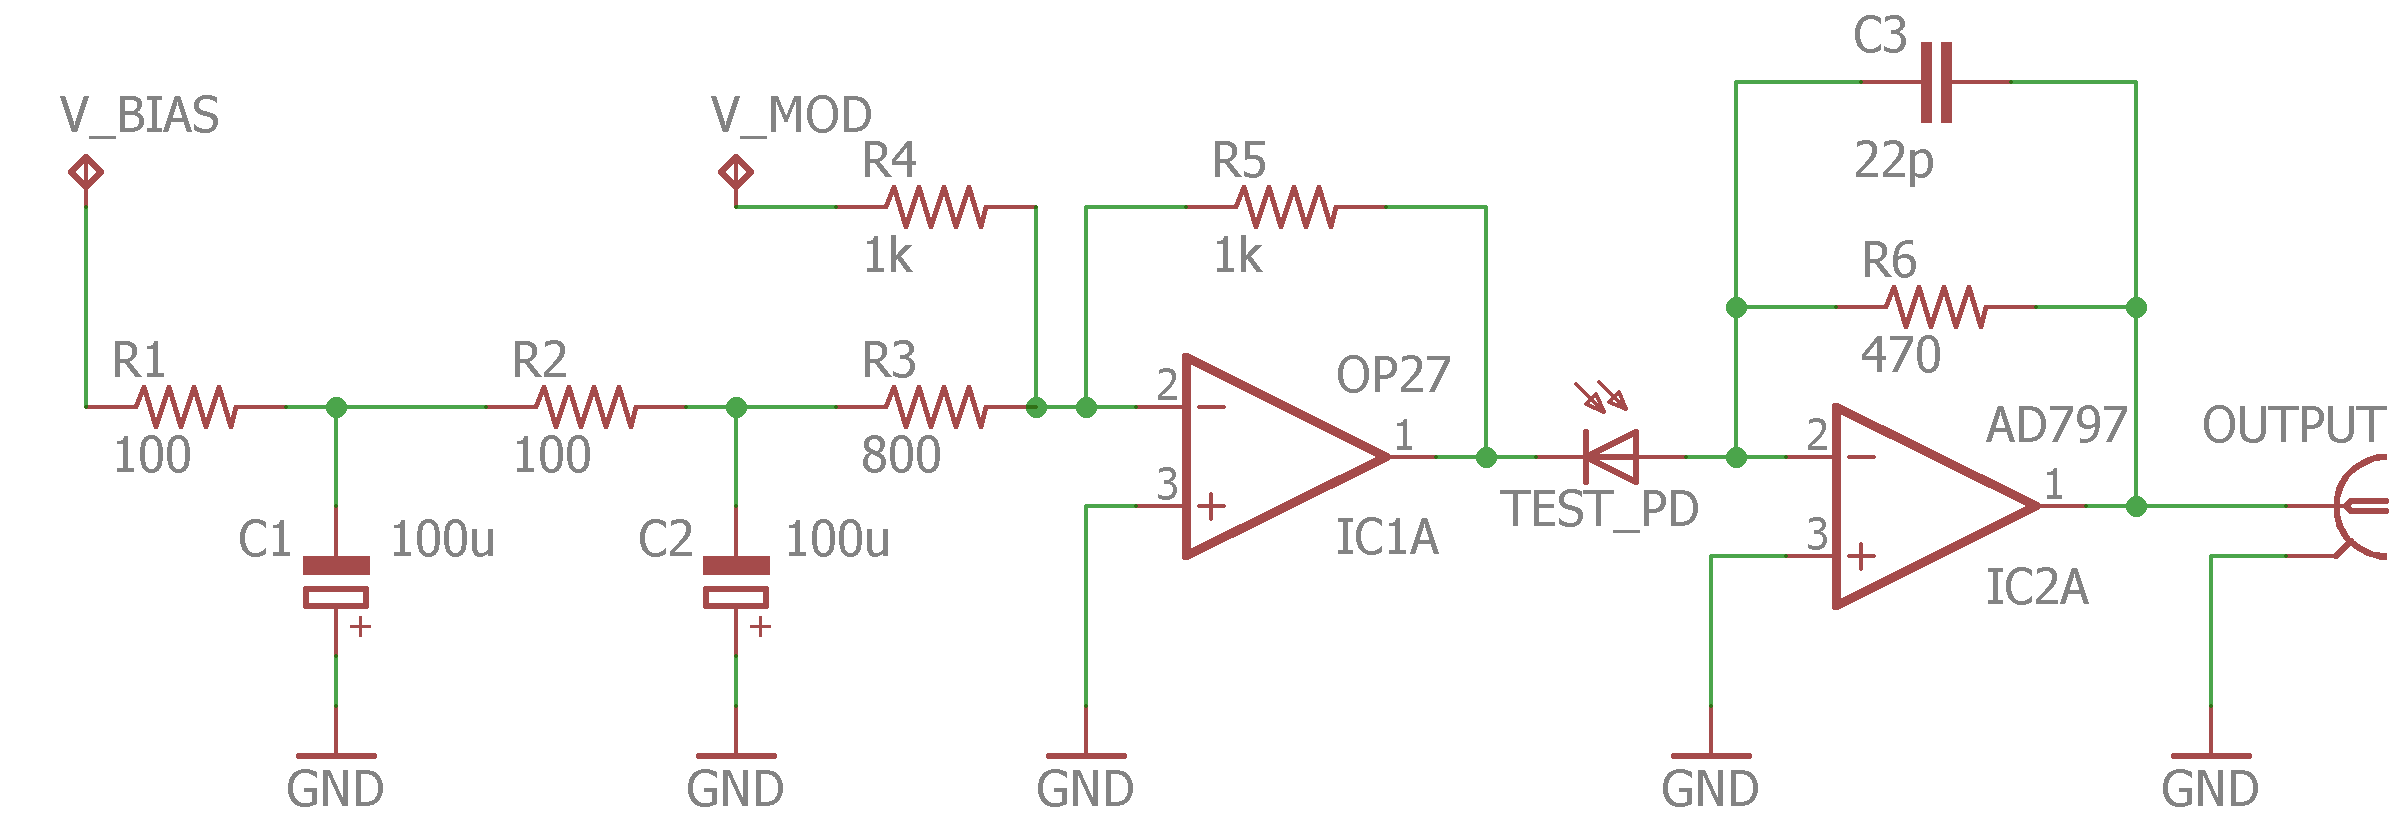
\includegraphics[width=0.9\linewidth]{qe_tester}
	\caption{Transimpedance amplifier used to measure the quantum efficiency and linearity of photodiodes for up to 20\,mW of 1550\,nm laser light. The reverse bias supplied to the photodiode is provided by the first OP amp (OP27). The two inputs $\mathrm{V_{bias}}$ and $\mathrm{V_{mod}}$ allows for a quiet low passed DC bias to be set while also being able to perform lock-in type measurements.}
	\label{fig:ad797pdtester}
\end{figure}
\begin{figure}
	\centering
	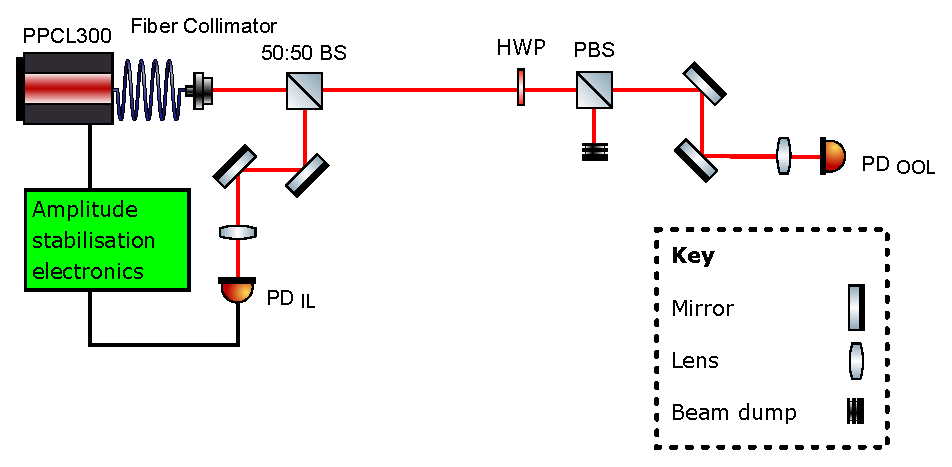
\includegraphics[width=0.7\linewidth]{test_set_up}
	\caption{Layout of experiment. PD\textsubscript{IL} is the in-loop photodiode (C30641gh) and PD\textsubscript{OOL} is the photodiode being tested. The PPCL300 is a 1550nm fibre laser from pure photonics. Since the C30641gh is a well-characterised diode, this was used as the in-loop diode for the amplitude stabilisation}
	\label{fig:testsetup}
\end{figure}

\section{Experimental Results from Testing Extended InGaAs Photodiodes.}
\paragraph{}
\begin{figure}[h]
	\centering
	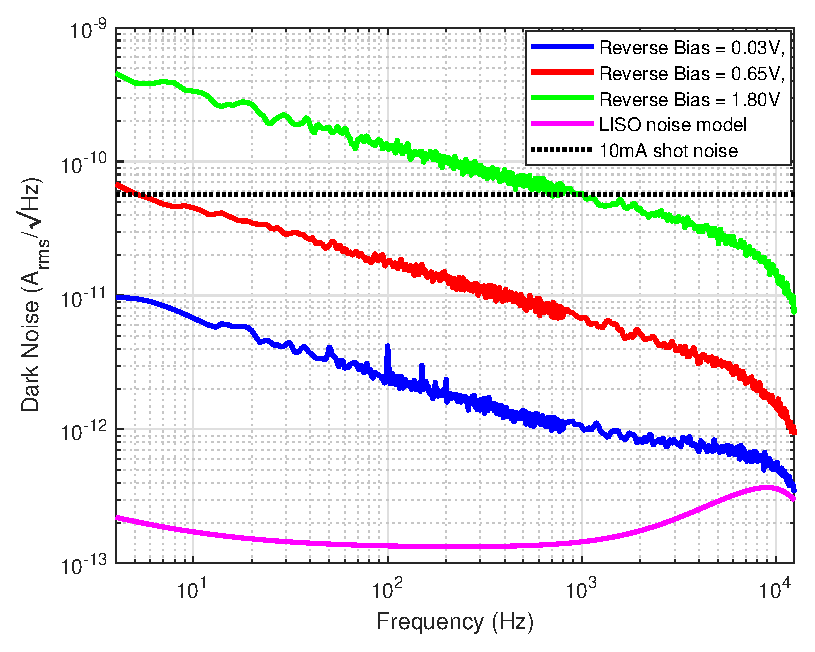
\includegraphics[width=0.7\linewidth]{fd10d_dark_noise_reverse_bias}
	\caption{The dark noise of the FD10D at different reverse biases. The maximum datasheet value is 1.8V, above this voltage electrons can start tunnelling across the band gap. The rolling off above \SIunits{9}{\,kHz} is an artefact of the circuit. Above 0.65\,V reverse bias, the $1/f$ noise becomes larger than shot noise. At this reverse bias, the quantum efficiency is $\sim$70\%. These measurements were made at room temperature.}
	\label{fig:fd10ddarknoisereversebias}
\end{figure}
\begin{figure}
	\centering
	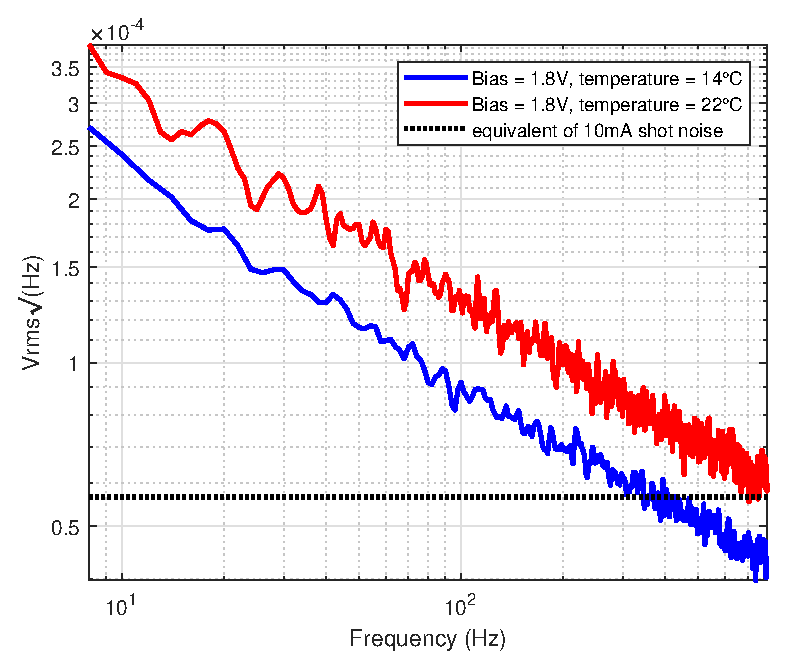
\includegraphics[width=0.7\linewidth]{cooling_fd10}
	\caption{The dark noise of the FD10D with a reverse bias of 1.8V at room temperature and 14\SIunits{\degree C}. Although there is a slight reduction in noise, this comes at the expense of less quantum efficiency near the cut off wavelength.}
	\label{fig:fd10ddarknoisetemp18v}
\end{figure}
The FD10D is a 1\,mm photodiode sold by Thorlabs, with a cut-off wavelength of 2.6\,\SIunits{\micro\metre}. Figure \ref{fig:dc11mw436um} shows why one would want to increase the bias as much as possible, as the amount of photo-current generated increases by 17\% for this particular diode when the reverse bias is turned up to its maximum data-sheet value \cite{FD10D}. The measured dark noise for this photodiode (see Figure \ref{fig:fd10ddarknoisereversebias}) shows that  running this diode with a reverse bias much higher than 0.65\,V would result in $1/f$ noise larger than the shot noise of a 10mA photo-current at the frequencies of interest ($\sim$100\,Hz). If used as a gravitational wave detector readout photodiode, the sensitivity of the detector would be limited by $1/f$ technical noise rather than quantum-limited noise floor of shot noise. The absolute quantum efficiency was measured for this diode using multiple power meters. Taking into account reflections from the glass window in front, the quantum efficiency was measured to be 82\% (the power of the laser was cross checked with 2 different power meters, these agreed to within less than 0.5\%) at 1.8\,V reverse bias. At 0.6\,V reverse bias the $1/f$ noise is below the target, but at he expense of the quantum efficiency which was measured to be 70\%. The maximum photo-current this diode was tested at 0.6V reverse bias was 15\,mA and this showed no sign of saturation. Although the FD10D did manage to handle a reasonable amount of power, the quantum efficiency was still far from the target of greater than 99\%.
\begin{figure}[h]
	\centering
	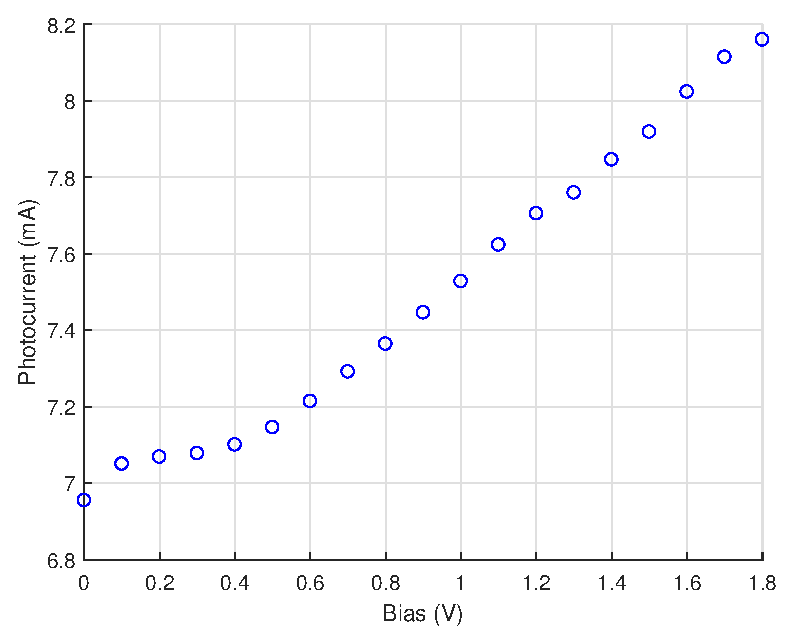
\includegraphics[width=0.7\linewidth]{DC_11mW_436um}
	\caption{A 1550\,nm laser was used to illuminate the FD10D at room temperature. As the reverse bias is increased, the photo-current out of the FD10D increases by about 17\%. This increase in photo-current is due to an increase quantum efficiency since the noise of photo-current matched shot noise.}
	\label{fig:dc11mw436um}
\end{figure}
\paragraph{}
It was necessary to check that the power-supply/bias voltage noise was not be effecting the result. In order to show the swappable photodiode design met the noise requirements, a fixed bias voltage with noise at 10Hz of 50\,$\text{nV}_{\mathrm{rms}}/\sqrt{\text{Hz}}$ was used to cross check the measurement of dark noise for the FD10D. This requirement was set by assuming that the dynamic impedance of the test photodiodes would be of the order 100\,\SIunits{\kilo\ohm}, and the smallest amount of current noise that is measurable at the inverting input of the TL071 in this circuit is 0.5\,$\text{pA}_{\mathrm{rms}}/\sqrt{\text{Hz}}$, so multiplying these two quantities gives the bias noise requirement. By having a socket rather than a solder joint and a standard voltage regulator to provide the bias, there is potential to have bias voltage noise of several 100\,$\text{uV}_{\mathrm{rms}}/\sqrt{\text{Hz}}$. A low noise reference voltage (AD587) with 2 low pass filters was used to create the quiet bias voltage (see Figure \ref{fig:darknoisetestbox2}). There was no difference in noise between using the swappable photodiode test circuit and the quiet bias voltage circuit (see Figure \ref{fig:bias_checks}), so we can rule out bias voltage noise being the cause of the $1/f$ noise. If the bias voltage produced $1/f$ noise and the photodiode also produced $1/f$ noise, then you would see a corner in the spectrum, as well as a generally messy looking spectrum. 
\begin{figure}[h]
	\centering
	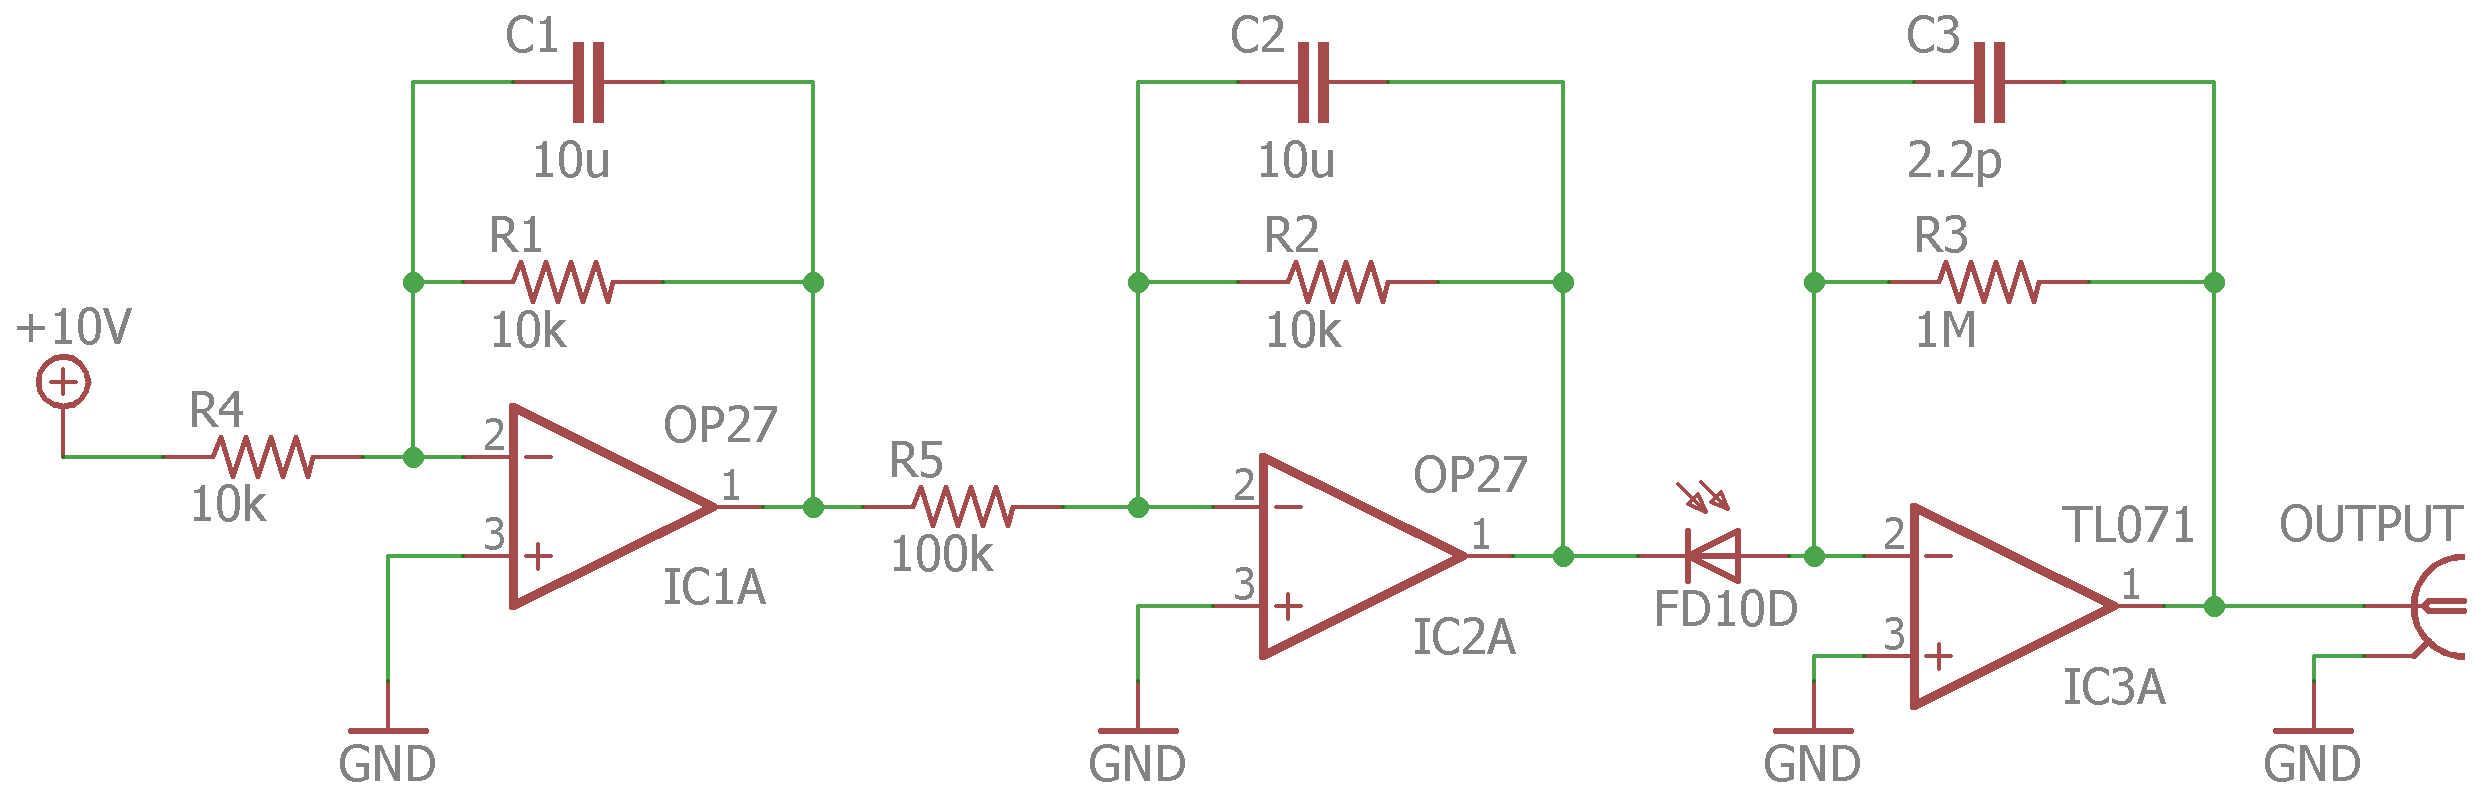
\includegraphics[width=0.7\linewidth]{dark_noise_test_box_2}
	\caption{Low noise fixed bias voltage dark noise measurement circuit. The 10V reference is generated by an AD587, in this circuit the noise is limited by the voltage noise of the second OP27, but it still reaches 5\,$\text{nV}_{\mathrm{rms}}/\sqrt{\text{Hz}}$ at \SIunits{10}{\,Hz} which is 10 times smaller than the amount of voltage noise which could be converted to current noise that would cause the signal at the output of the TL071 not to be limited by the current noise of the TL071, given the typical dynamic impedance for extended InGaAs photodiodes.}
	\label{fig:darknoisetestbox2}
\end{figure}

\begin{figure}[h]
	\centering
	\begin{subfigure}{0.5\textwidth}
		\centering
		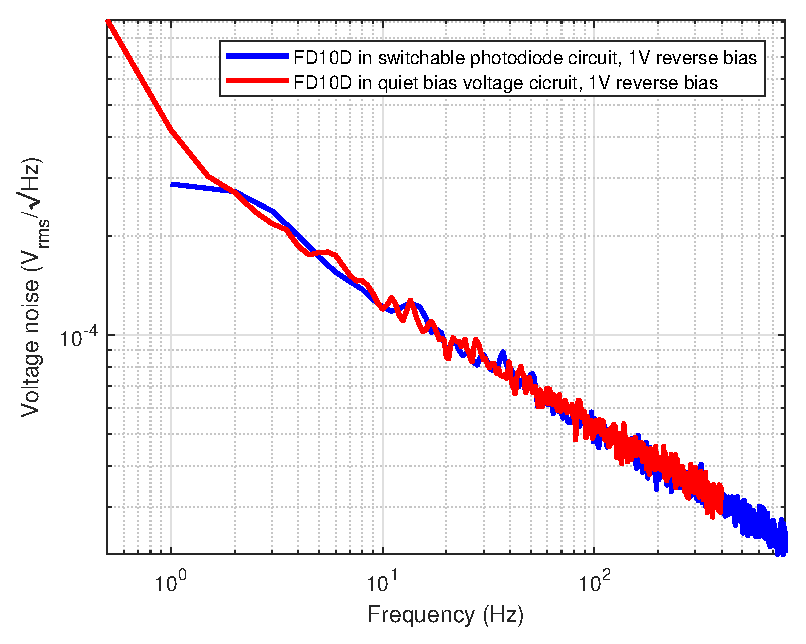
\includegraphics[width=1\linewidth]{cross_check}
		\caption{}
		\label{fig:cross_check}
	\end{subfigure}%
	\begin{subfigure}{0.5\textwidth}
		\centering
		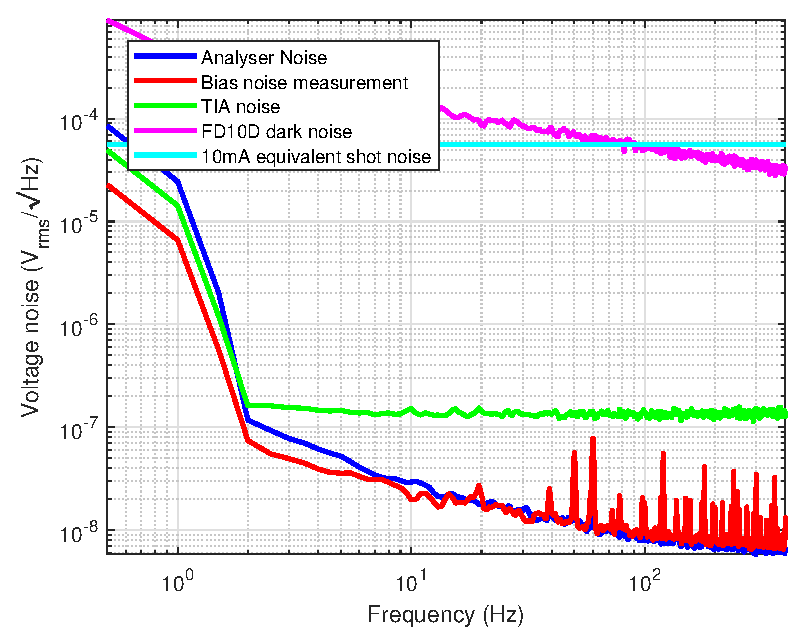
\includegraphics[width=1\linewidth]{FD10D_dark_noise_1V_noise_sources}
		\caption{}
		\label{fig:FD10D_dark_noise_1V_noise_sources}
	\end{subfigure}
	\caption{The left panel shows that the quiet reverse bias voltage source, shown in figure \ref{fig:darknoisetestbox2}, and the more noisy but more flexible bias voltage source, shown in figure \ref{fig:tl071}, gave the same results when the dark noise of the FD10D was measured. This means that the flexible reverse bias source is suitable to use for measuring the dark noise of other photodiodes. The bias voltage noise in the quiet bias voltage circuit was found to meet the requirements as shown in the right panel.}
	\label{fig:bias_checks}
\end{figure}
\paragraph{}
The large amounts of $1/f$ noise was not unique to the FD10D - several extended InGaAs photodiodes from Laser Components were also tested. The main problem was the $1/f$ noise becoming large whenever the bias voltage was increased in an attempt to improve the quantum efficiency, necessitating the use a small reverse bias. A small reverse bias results in electrons-hole pairs failing to make it out of the junction before recombining, leading to a smaller quantum efficiency as well as causing the photodiode to saturate. The Laser Components extended InGaAs photodiodes that were tested performed poorly in both noise and power handling terms (see Figures \ref{fig:lasercomponentsnoise} and \ref{fig:ratio}).
\begin{figure}[h]
	\centering
	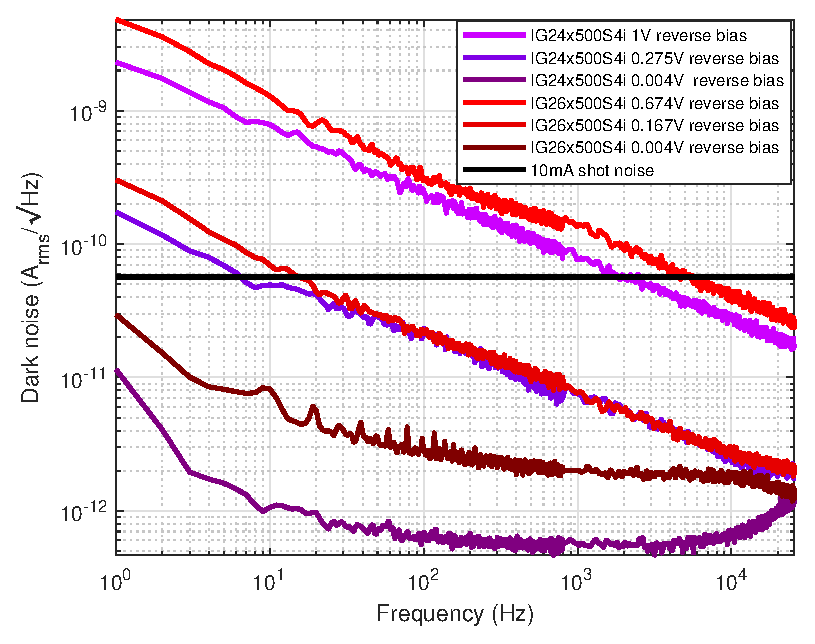
\includegraphics[width=0.7\linewidth]{laser_components_noise}
	\caption{The dark noise of two different extended InGaAs photodiodes from Laser Components measured at room temperature. The noise curve for the IG24x500S4i at 0.004V is limited by the noise of the circuit shown in Figure \ref{fig:tl071}. As the reverse bias is reduced, so is the $1/f$ noise. The IG26x500S4i had to be used at a lower reverse bias than the IG24x500S4i to achieve the same noise performance.}
	\label{fig:lasercomponentsnoise}
\end{figure}
\begin{figure}[h]
	\centering
	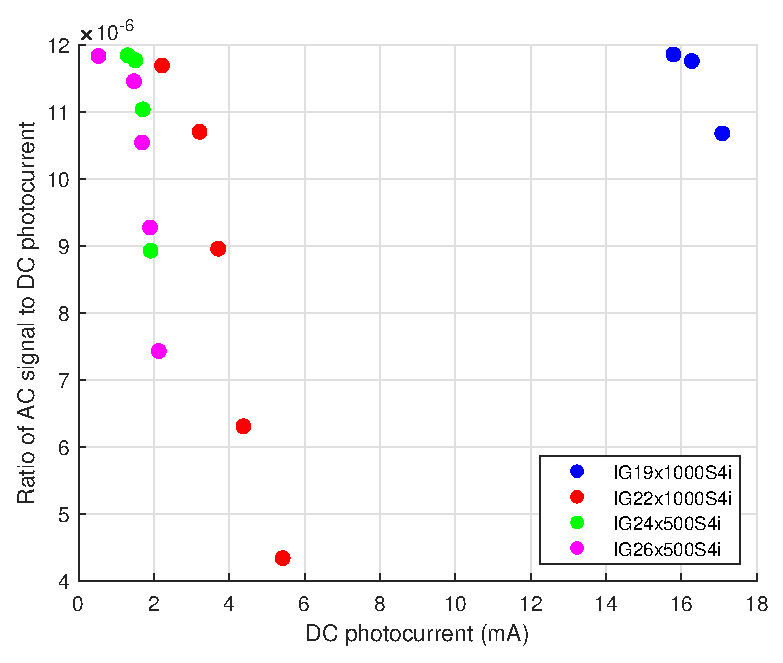
\includegraphics[width=0.7\linewidth]{ratio}
	\caption{Using the apparatus shown in figure \ref{fig:testsetup}, the DC photo-current that the Laser Components extended InGaAs photodiodes could be operated with while still being linear (i.e. the AC component of the signal would scale linearly with the DC photo-current) was investigated. The spot size on the photodiodes was made as large as possible while still containing 99\% of the light power on the photodiode, and were operated with the maximum reverse bias voltage that would still give $1/f$ noise less than 10mW shot noise at the frequencies of interest for the a gravitational wave detector. The laser's amplitude was modulated. Using a lock-in technique the AC response was measured and divided by the DC photo-current. This was compared to the AC/DC response of the in-loop regular InGaAs photodiode which behaved linearly. When the AC/DC ratio starts to become smaller, the photodiode is no longer behaving linearly. As these diodes become more extended, they perform more poorly.}
	\label{fig:ratio}
\end{figure}
\paragraph{}
To investigate the physical mechanism of the $1/f$ noise found in extended InGaAs photodiodes, the forward current voltage curve of the IG24x500S4i was investigated. The ideality factor, $n$, of a diode indicates the process by which the generation-recombination current is created. The ideality factor of the IG24x500S4i was measured using the apparatus shown in Figure \ref{fig:tl071} and compared to the model 
\begin{equation}
I = I_s(e^{-qV/nk_BT}-1)
\label{model}
\end{equation}
where $I_s$ is the saturation current, $q$ is the electron charge, $V$ is the voltage across the diode, $k_B$ is the Boltzmann constant and $T$ is the temperature. An ideality factor of 1 suggests that the generation-recombination current is driven by the existence of trap states (rather than a multi electron-hole process). This is shown in Figure \ref{fig:forwardbiasiv}. Fitting for $I_s$ and $n$ gives the saturation current to be 0.36\,mA and the ideality factor to be 1.02.
\section{Conclusion}
\begin{figure}
	\centering
	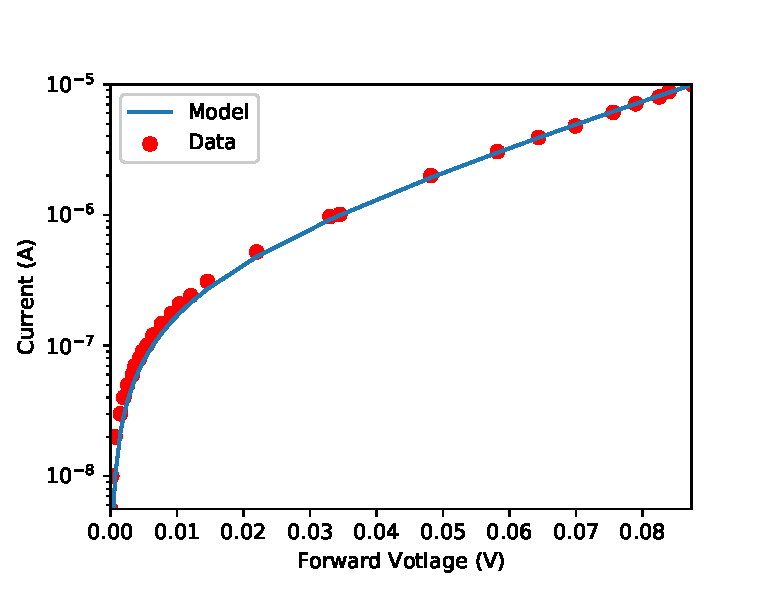
\includegraphics[width=0.7\linewidth]{forward_bias_IV}
	\caption{The forward IV curve of the IG24x500S4i.}
	\label{fig:forwardbiasiv}
\end{figure}
Current off-the-shelf extended InGaAs photodiodes do not meet the requirements for readout schemes of future gravitational wave detectors given that simple PIN extended InGaAs photodiode diodes at room temperature are either too noisy, cannot handle enough power or do not have a high enough quantum efficiency. To overcome $1/f$ noise either a low bias is required which reduces the quantum efficiency, or a sophisticated modulation-demodulation scheme compatible with squeezing is required. A lower bias results in photons not being detected which detriments the amount of squeezing one can achieve, as does non-optimal chopping. With careful design of the layers within the photodiode and choice of fabrication process, the strain induced threading dislocations can be reduced, although suppliers of extended InGaAs photodiodes do not offer much hope when asked if a photodiode that meets the requirement of a third generation gravitational wave detector can be produced. The decision to run third generation detectors at 2\,\SIunits{\micro\metre} relies on being able get high quantum efficiency, low noise photodiodes. Non-extended InGaAs photodiodes such as the ones used by LIGO would be compatible with using a 1550\,nm laser. Other photodiode materials that are sensitive to 2\,\SIunits{\micro\metre} such as InSb and HgCeTd should also be investigated in terms of use for the read out of a gravitational wave detector. %A possible material for detecting 2\,\SIunits{\micro\metre} light is germanium however these diodes have low shunt resistances and high dark current. HgCdTe could also be used as reference \cite{TeledyneMCT} indicates that detectors with 94\% quantum efficiency and have noise equivalent powers even at room temperature well below the shot noise requirement of LIGO can be created, however this needs further investigation.
\section{Acknowledgements}
I would like to thank Andrew Long for our useful discussion about InGaAs, Sean Leavey for discussions about photodiodes, and Sebastian Steinlechner for providing us with some Laser Components photodiodes to test.

\chapter{Conclusion and Future Work}
\appendix
\chapter{Control Theory}
\bibliography{C:/bibliography/bibliography}
\end{document}